\chapter{Study Monitor}

This chapter explains how to use the Study Monitor application.

\section{Homepage}

Figure \ref{fig:study_homepage}.

\begin{figure}[H]
    \centering
    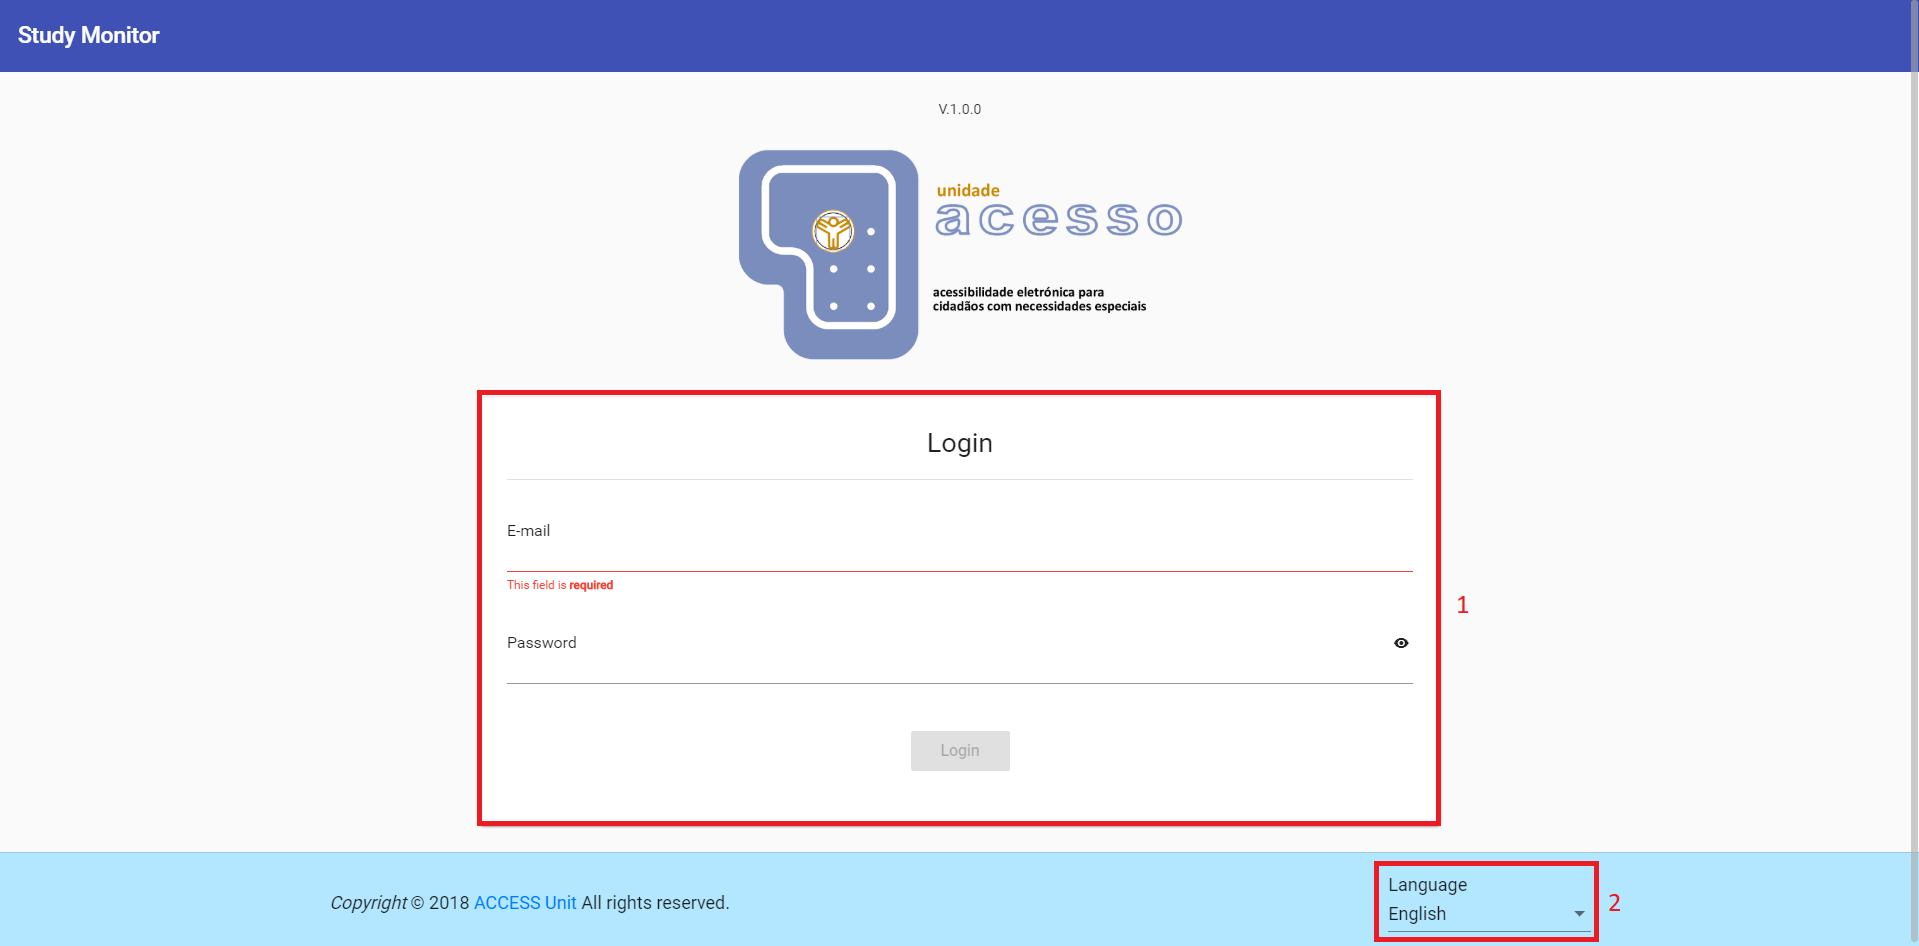
\includegraphics[width=\linewidth]{lib/images/study/study_homepage.png}
    \caption{Study Monitor homepage}
    \label{fig:study_homepage}
\end{figure}

\begin{enumerate}
    \item Login form
    \item Language selection box
\end{enumerate}

\section{List of categories page}

Figures \ref{fig:study_list_categories_page_empty} - \ref{fig:study_list_categories_page_full}.

\begin{figure}[H]
    \centering
    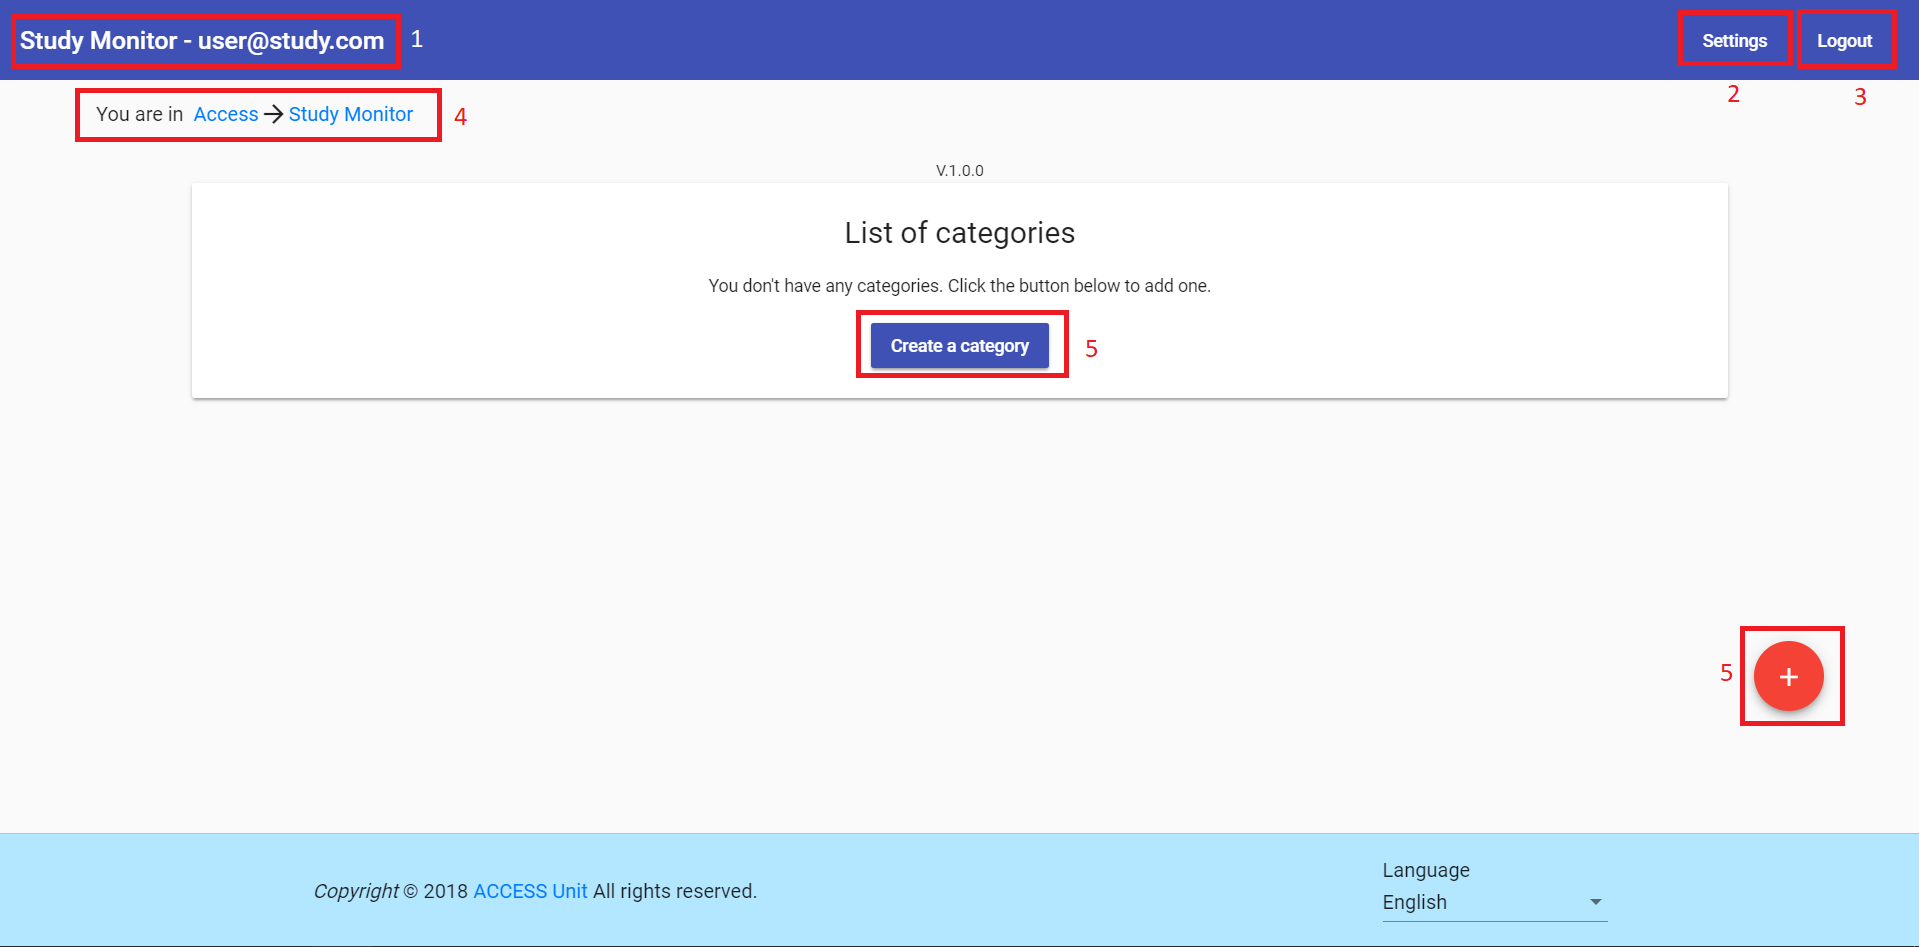
\includegraphics[width=\linewidth]{lib/images/study/study_list_categories_page_empty.png}
    \caption{Study Monitor list of categories page}
    \label{fig:study_list_categories_page_empty}
\end{figure}

\begin{figure}[H]
    \centering
    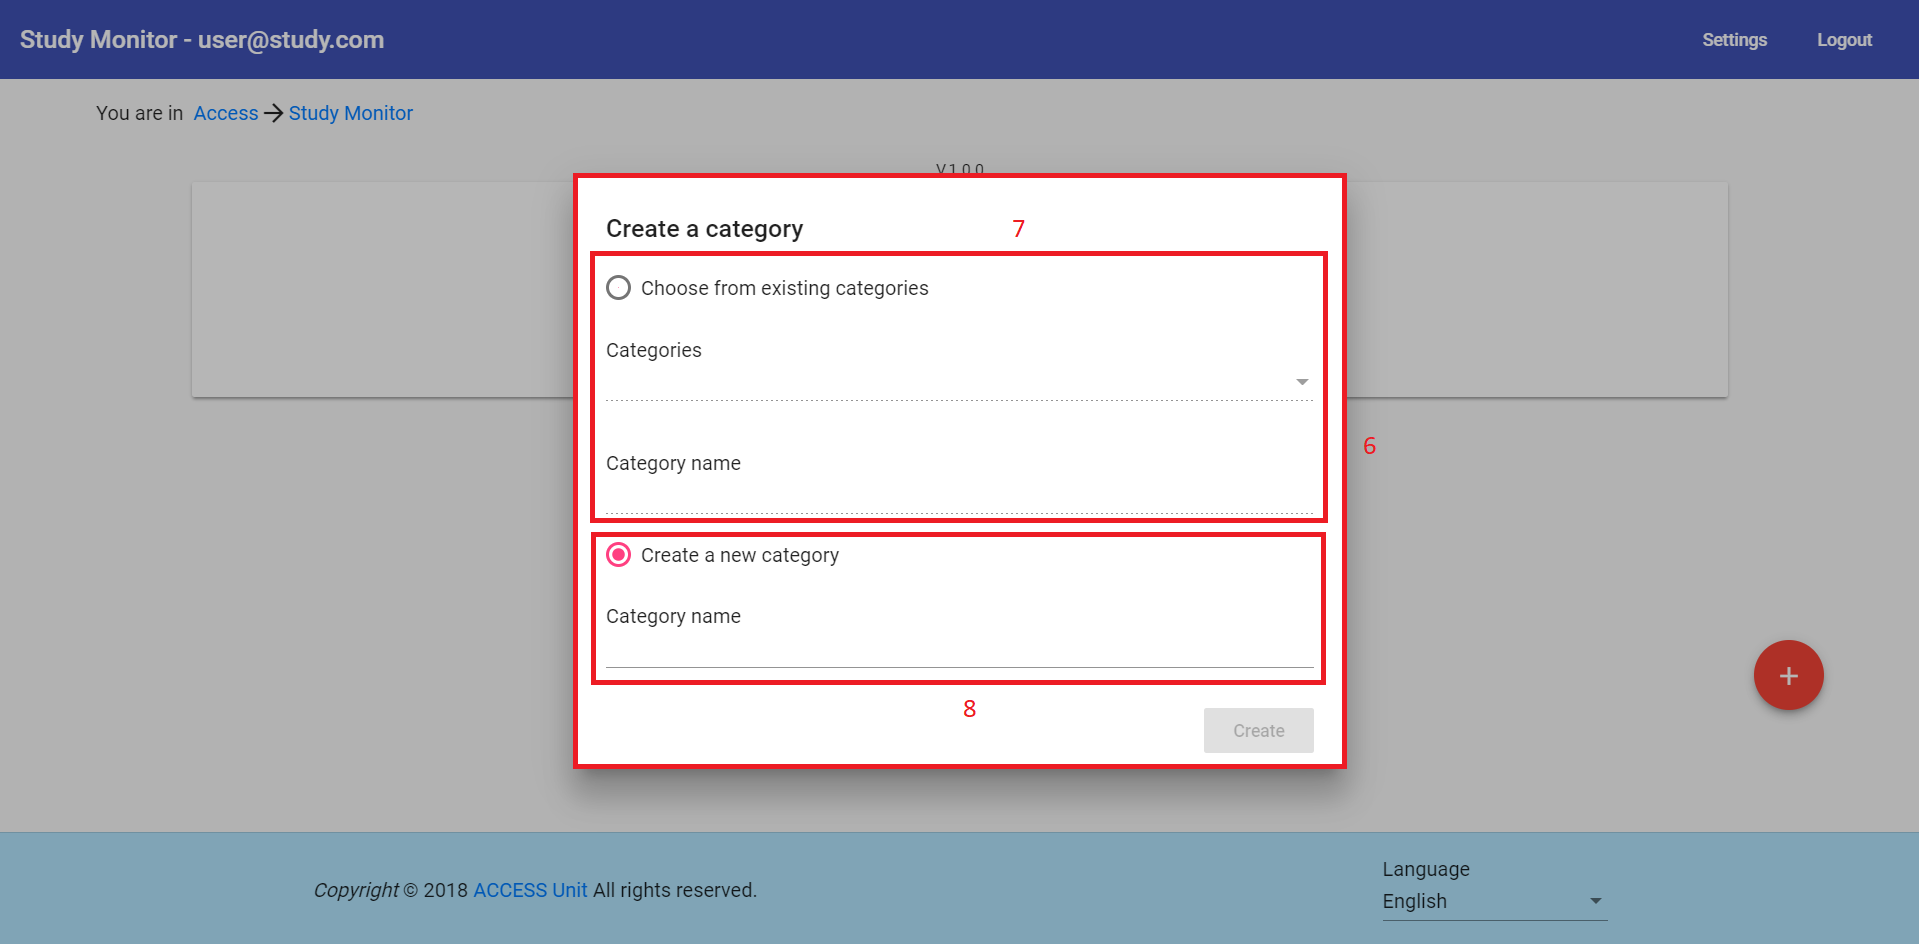
\includegraphics[width=\linewidth]{lib/images/study/study_create_category.png}
    \caption{Study Monitor create category}
    \label{fig:study_list_categories_page_create}
\end{figure}

\begin{figure}[H]
    \centering
    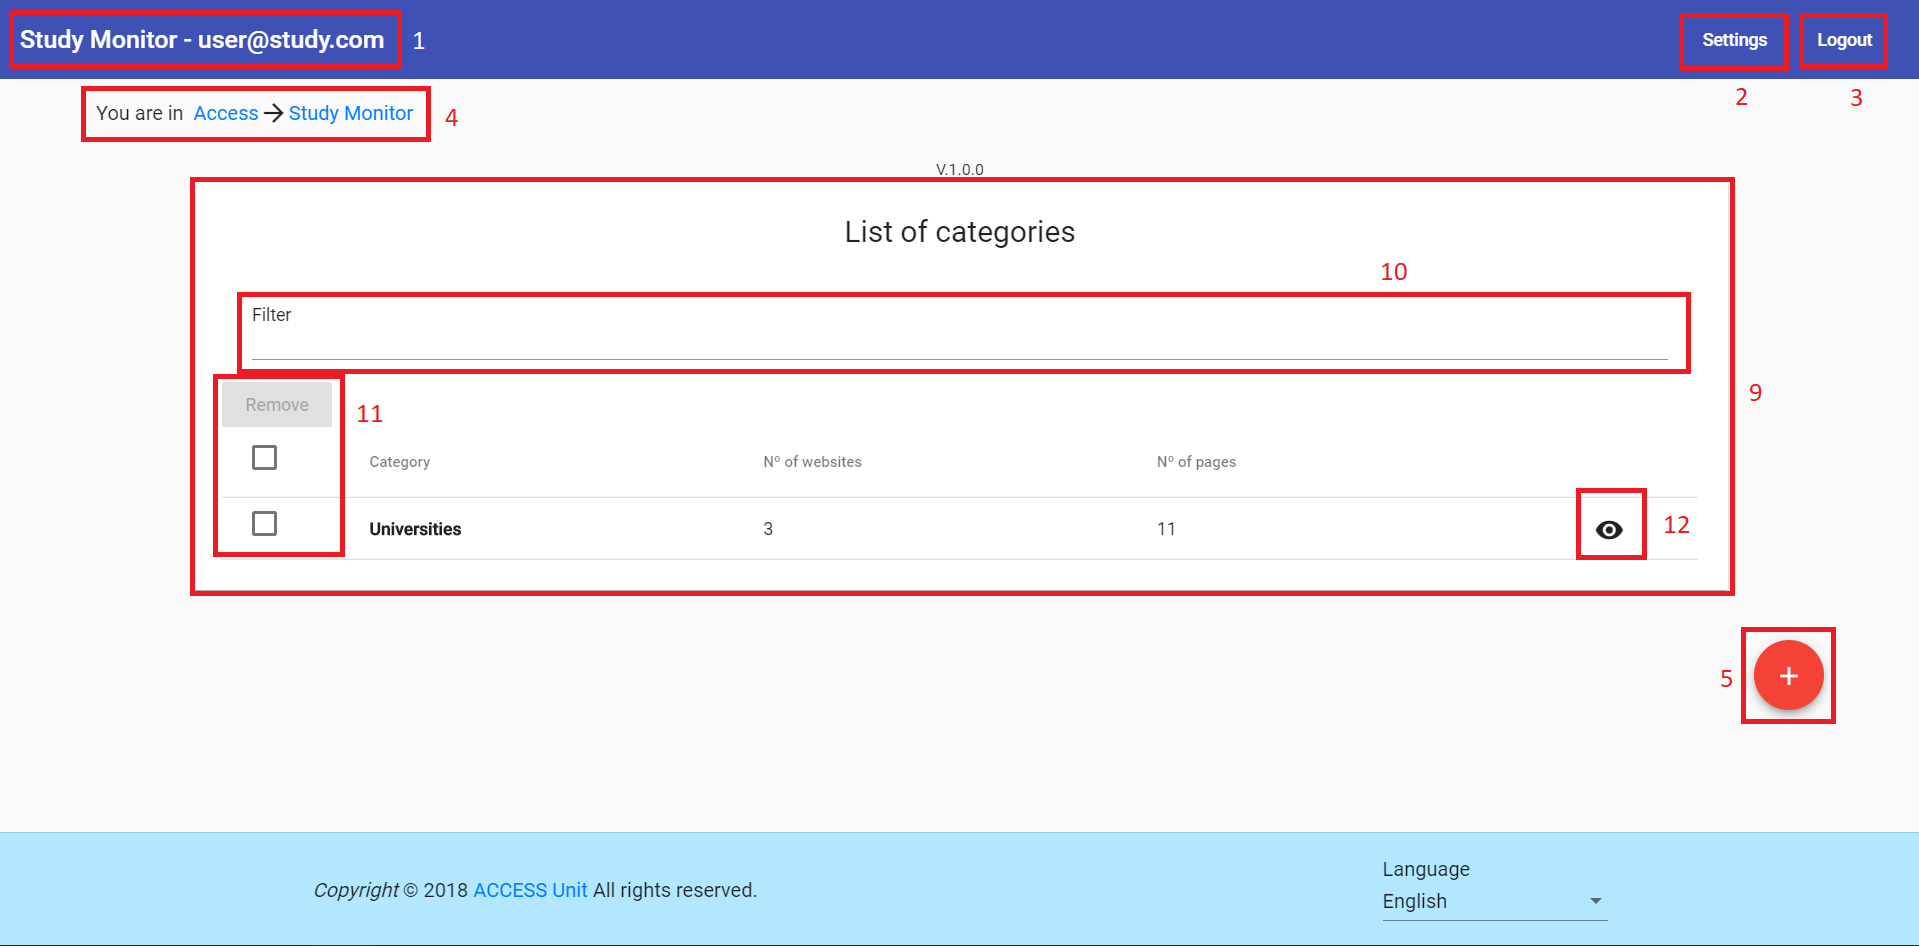
\includegraphics[width=\linewidth]{lib/images/study/study_list_categories_page_full.png}
    \caption{Study Monitor list of categories page}
    \label{fig:study_list_categories_page_full}
\end{figure}

\begin{enumerate}
    \item User account email
    \item Go to account settings
    \item Logs out the user
    \item Breadcrumbs menu
    \item Opens the ``Create category'' dialog
    \item ``Create category'' dialog
    \item Create a category from existing categories
    \item Create a new empty category
    \item List o user categories
    \item List of categories filter
    \item Remove categories
    \item See category information
\end{enumerate}

\section{Settings page}

Check My Monitor settings page, section \ref{sec:monitor_settings_page}.

\section{Category page}

Figures \ref{fig:study_category_page} - \ref{fig:study_category_page_3}.

\begin{figure}[H]
    \centering
    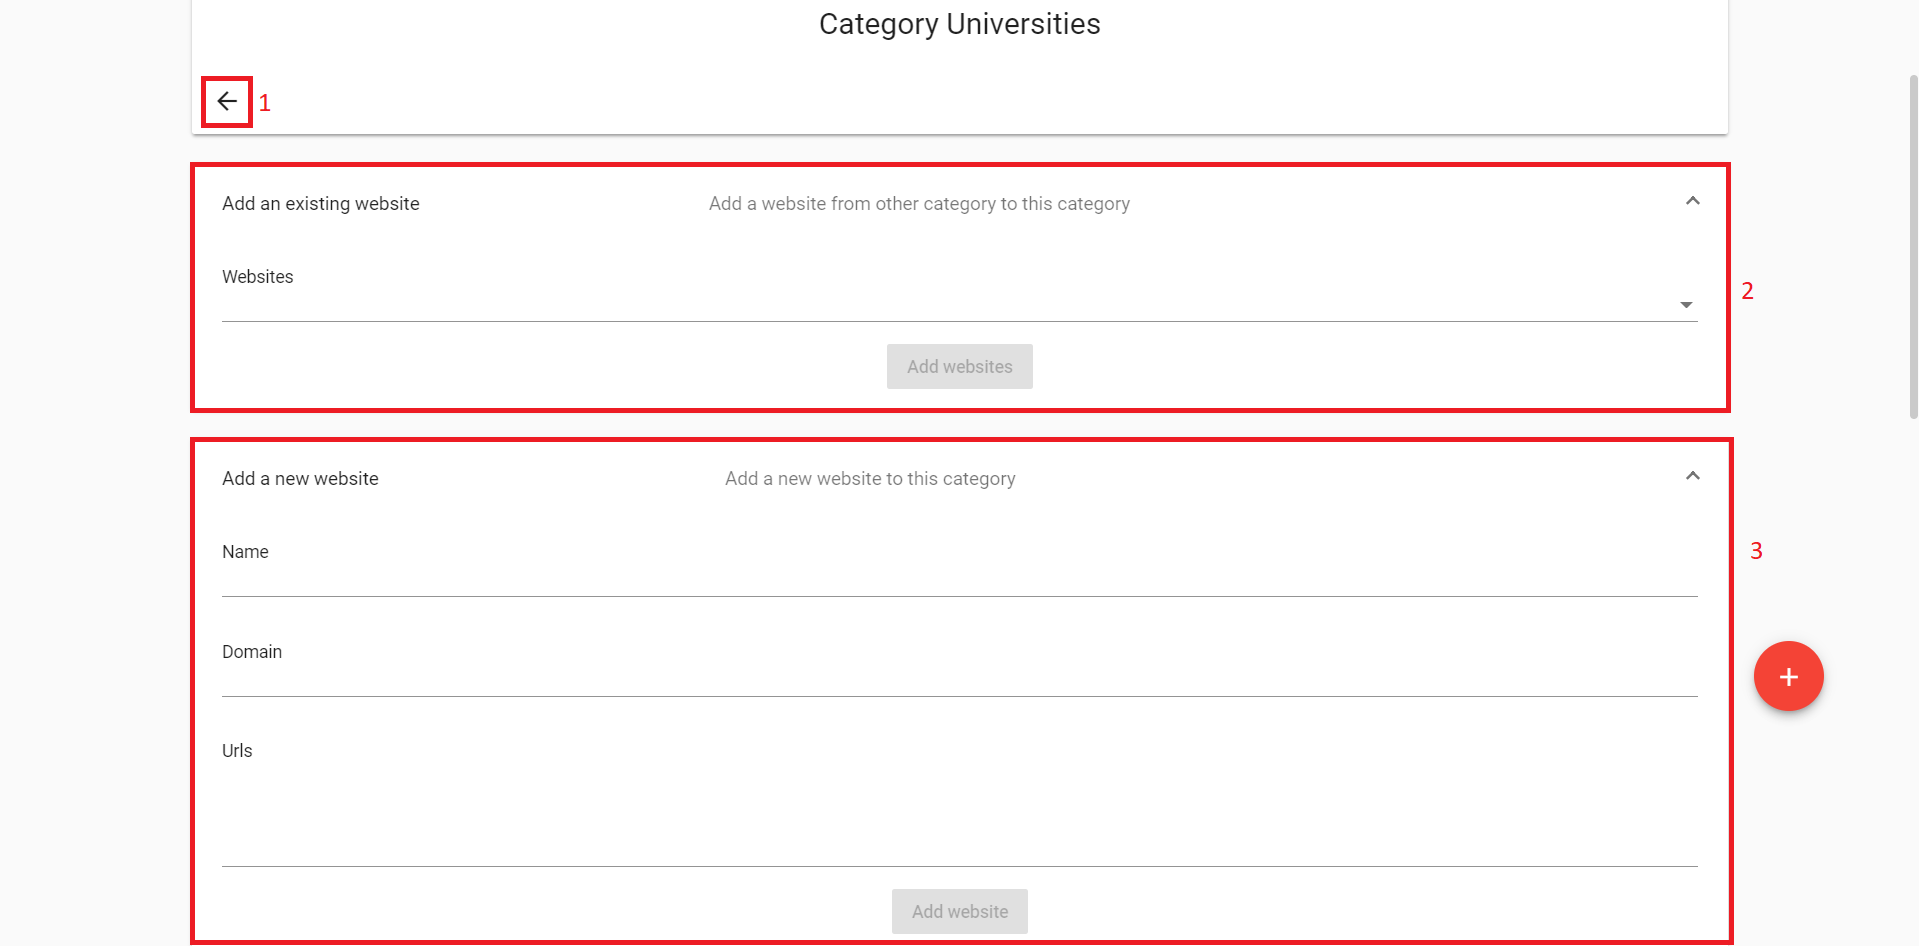
\includegraphics[width=\linewidth]{lib/images/study/study_category_page.png}
    \caption{Study Monitor category page}
    \label{fig:study_category_page}
\end{figure}

\clearpage

\begin{figure}[H]
    \centering
    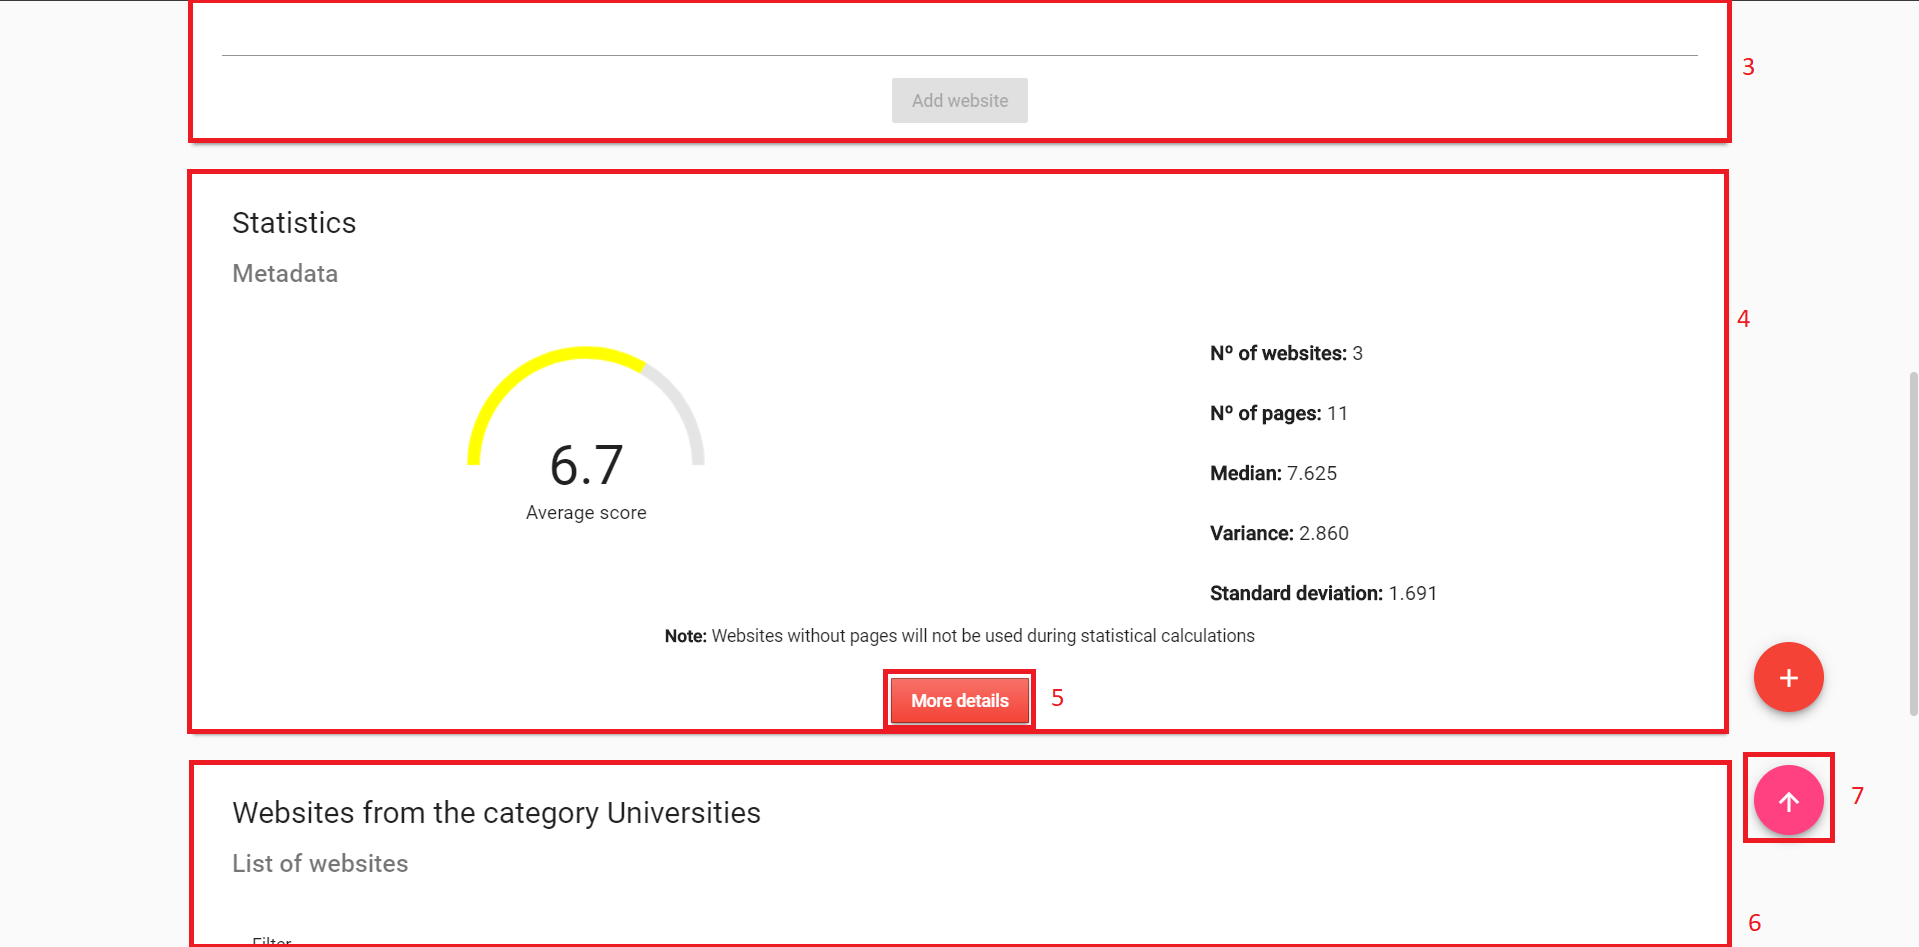
\includegraphics[width=\linewidth]{lib/images/study/study_category_page_2.png}
    \caption{Study Monitor category page (cont.)}
    \label{fig:study_category_page_2}
\end{figure}

\begin{figure}[H]
    \centering
    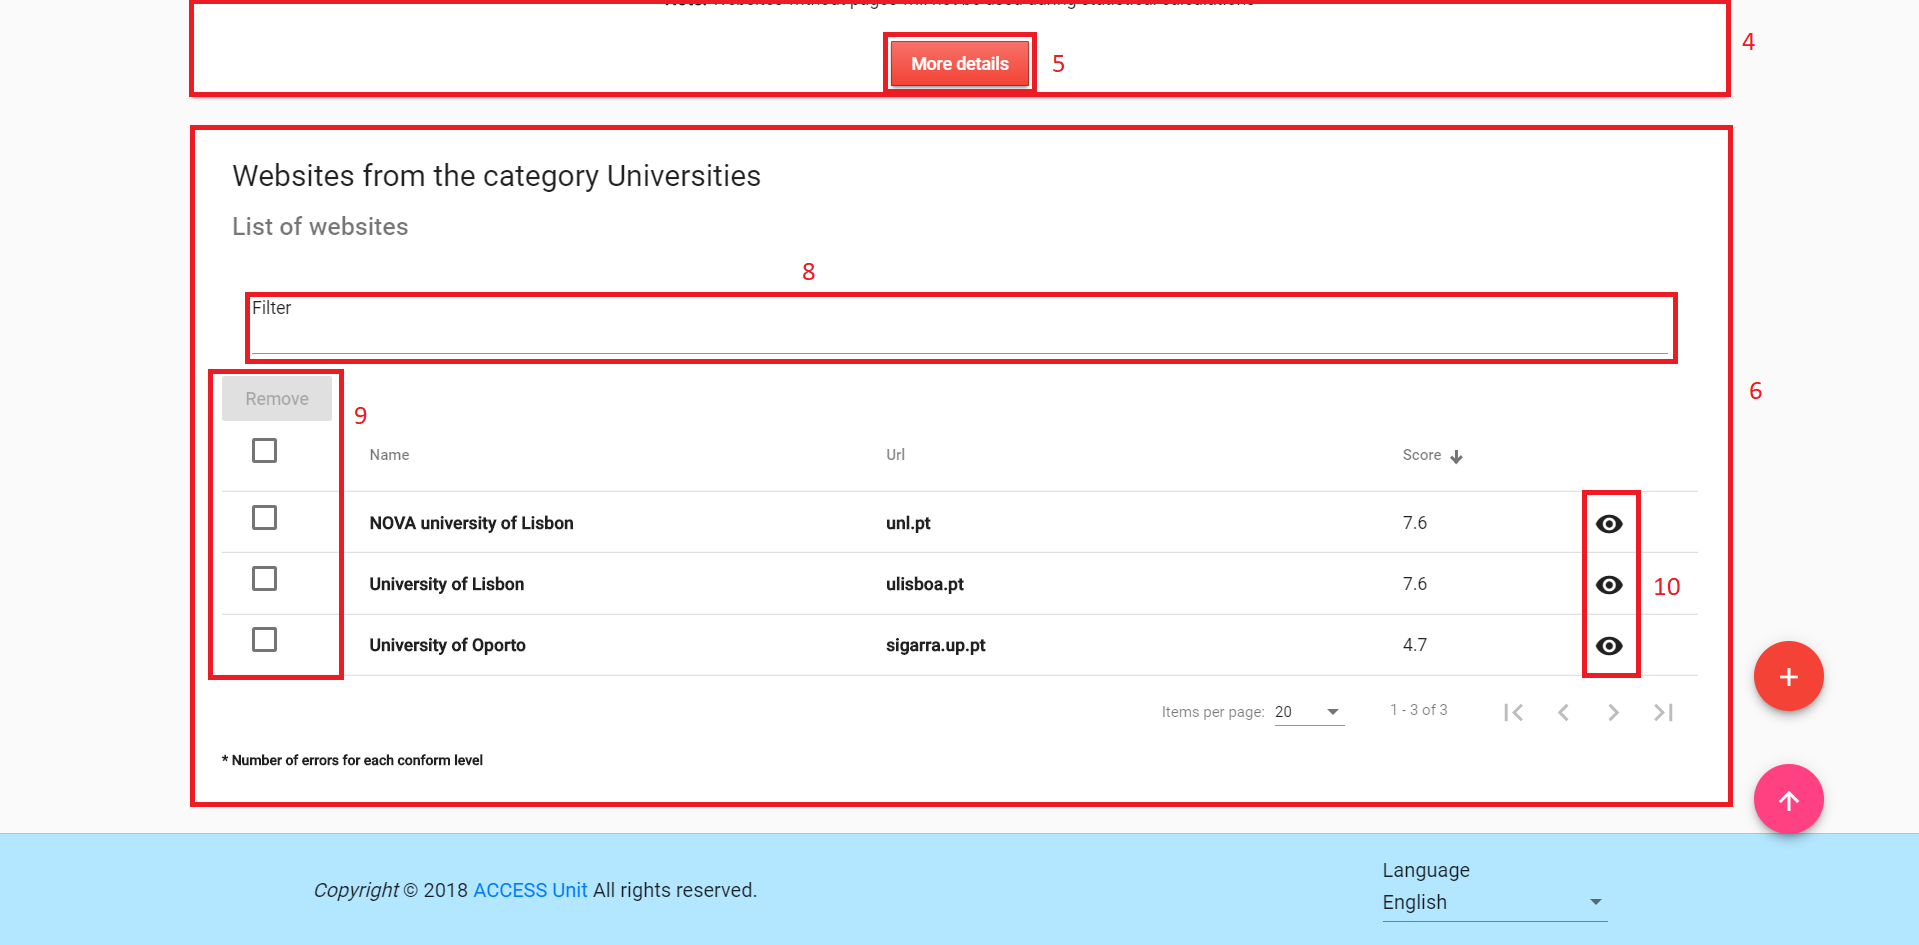
\includegraphics[width=\linewidth]{lib/images/study/study_category_page_3.png}
    \caption{Study Monitor category page (cont.)}
    \label{fig:study_category_page_3}
\end{figure}

\begin{enumerate}
    \item Goes back to the previous page (list of categories page)
    \item Add a website from other category to the current category form
    \item Add a new website to the current category form
    \item Category general statistics
    \item Go to ``Category detailed statistics'' page
    \item List of category websites
    \item ``Go to top'' button
    \item Category websites filter
    \item Remove websites from category
    \item See website information
\end{enumerate}

\section{Category statistics page}

Figures \ref{fig:study_category_statistics_page} - \ref{fig:study_category_statistics_page_5}.

\begin{figure}[H]
    \centering
    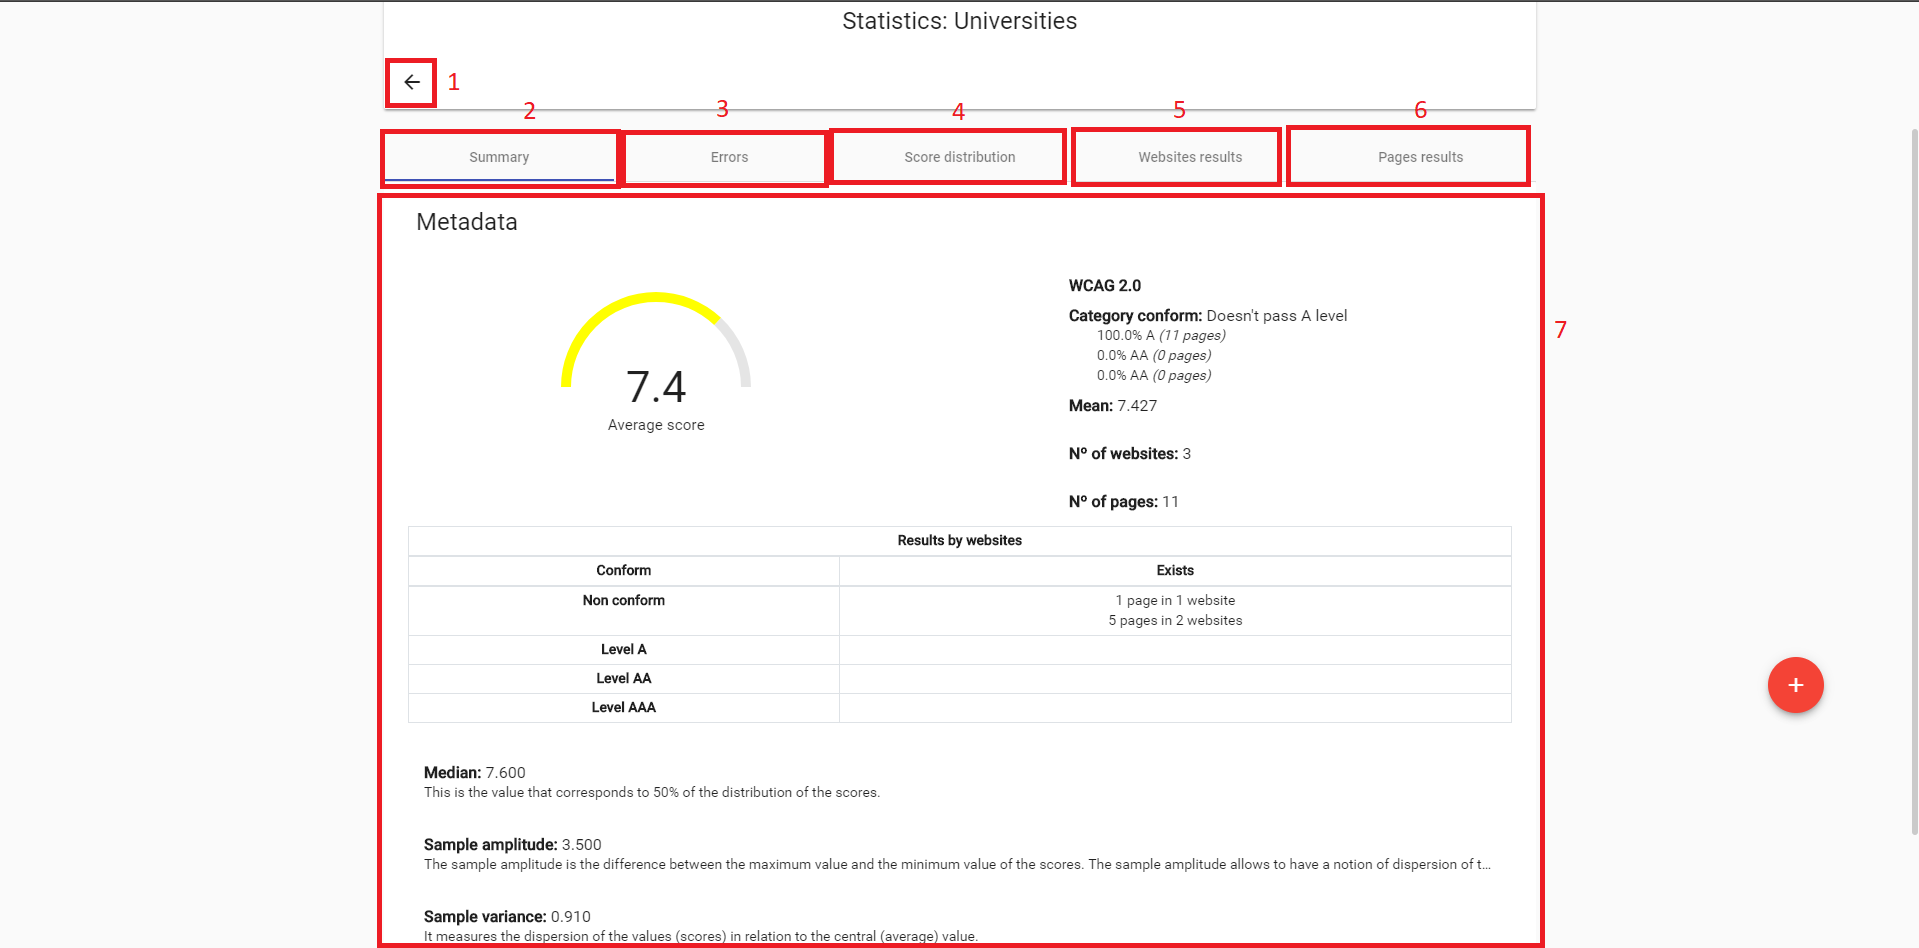
\includegraphics[width=\linewidth]{lib/images/study/study_category_statistics.png}
    \caption{Study Monitor category statistics page}
    \label{fig:study_category_statistics_page}
\end{figure}

\clearpage

\begin{figure}[H]
    \centering
    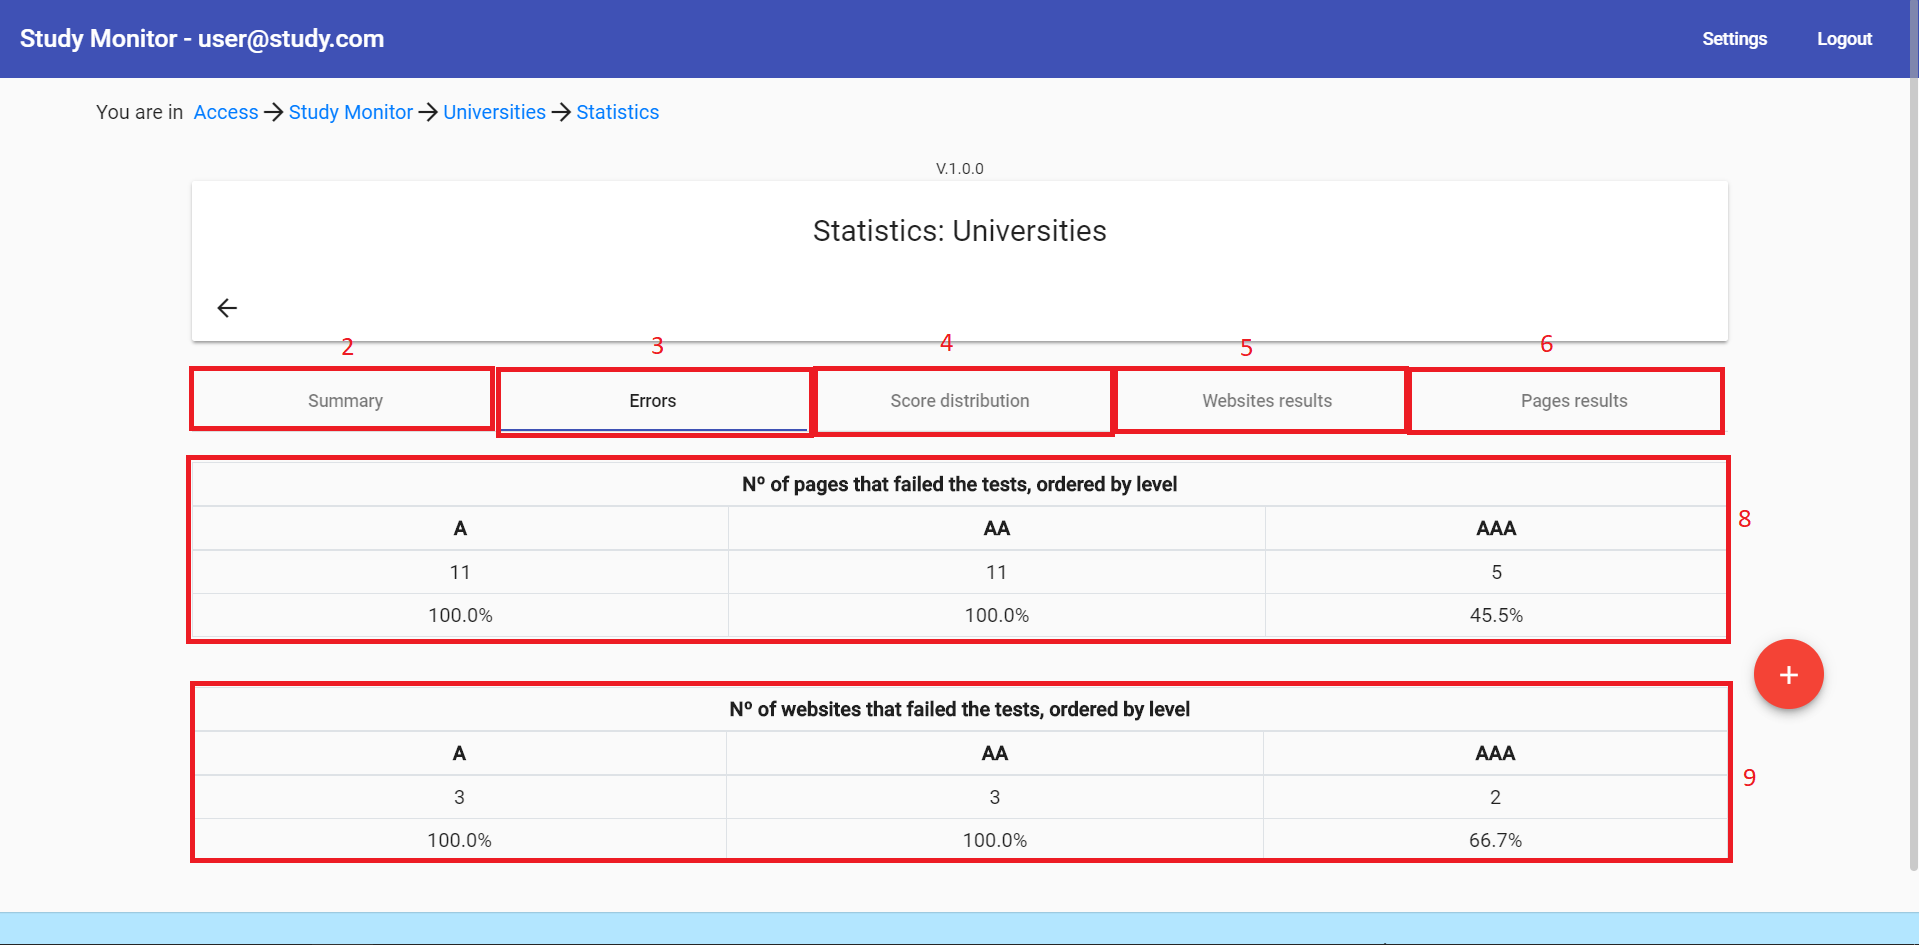
\includegraphics[width=\linewidth]{lib/images/study/study_category_statistics_2.png}
    \caption{Study Monitor category statistics page (cont.)}
    \label{fig:study_category_statistics_page_2}
\end{figure}

\begin{figure}[H]
    \centering
    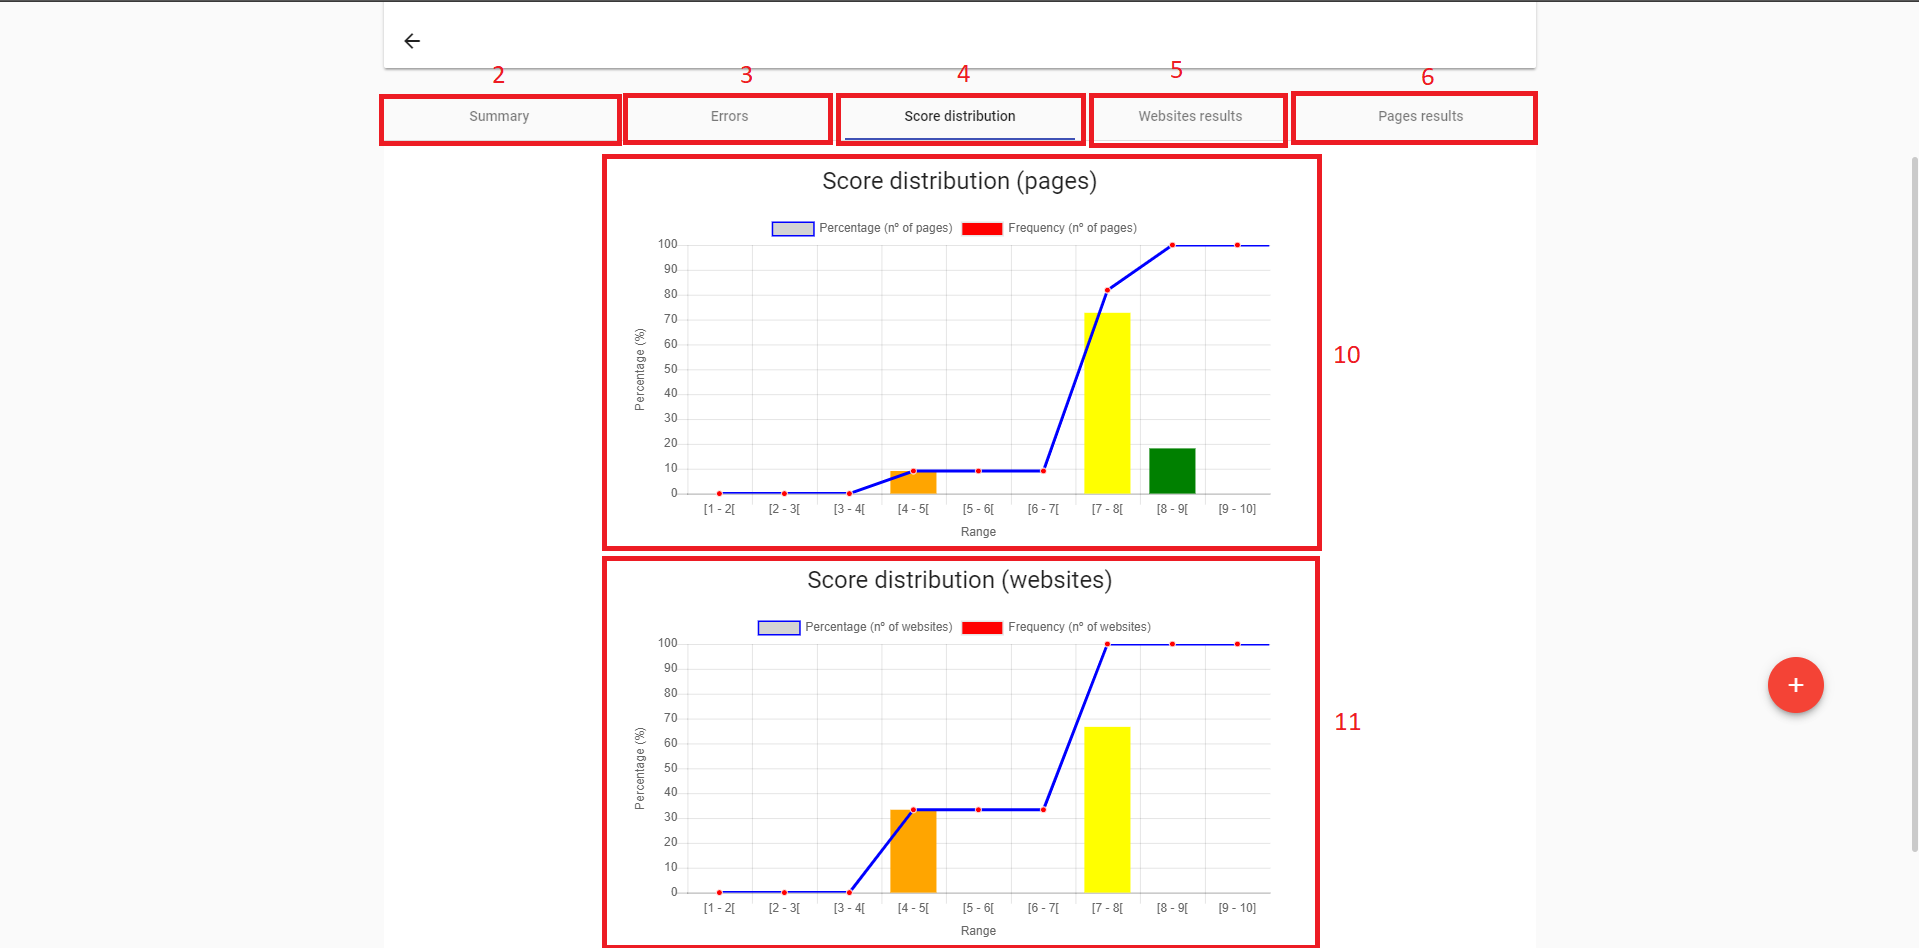
\includegraphics[width=\linewidth]{lib/images/study/study_category_statistics_3.png}
    \caption{Study Monitor category statistics page (cont.)}
    \label{fig:study_category_statistics_page_3}
\end{figure}

\begin{figure}[H]
    \centering
    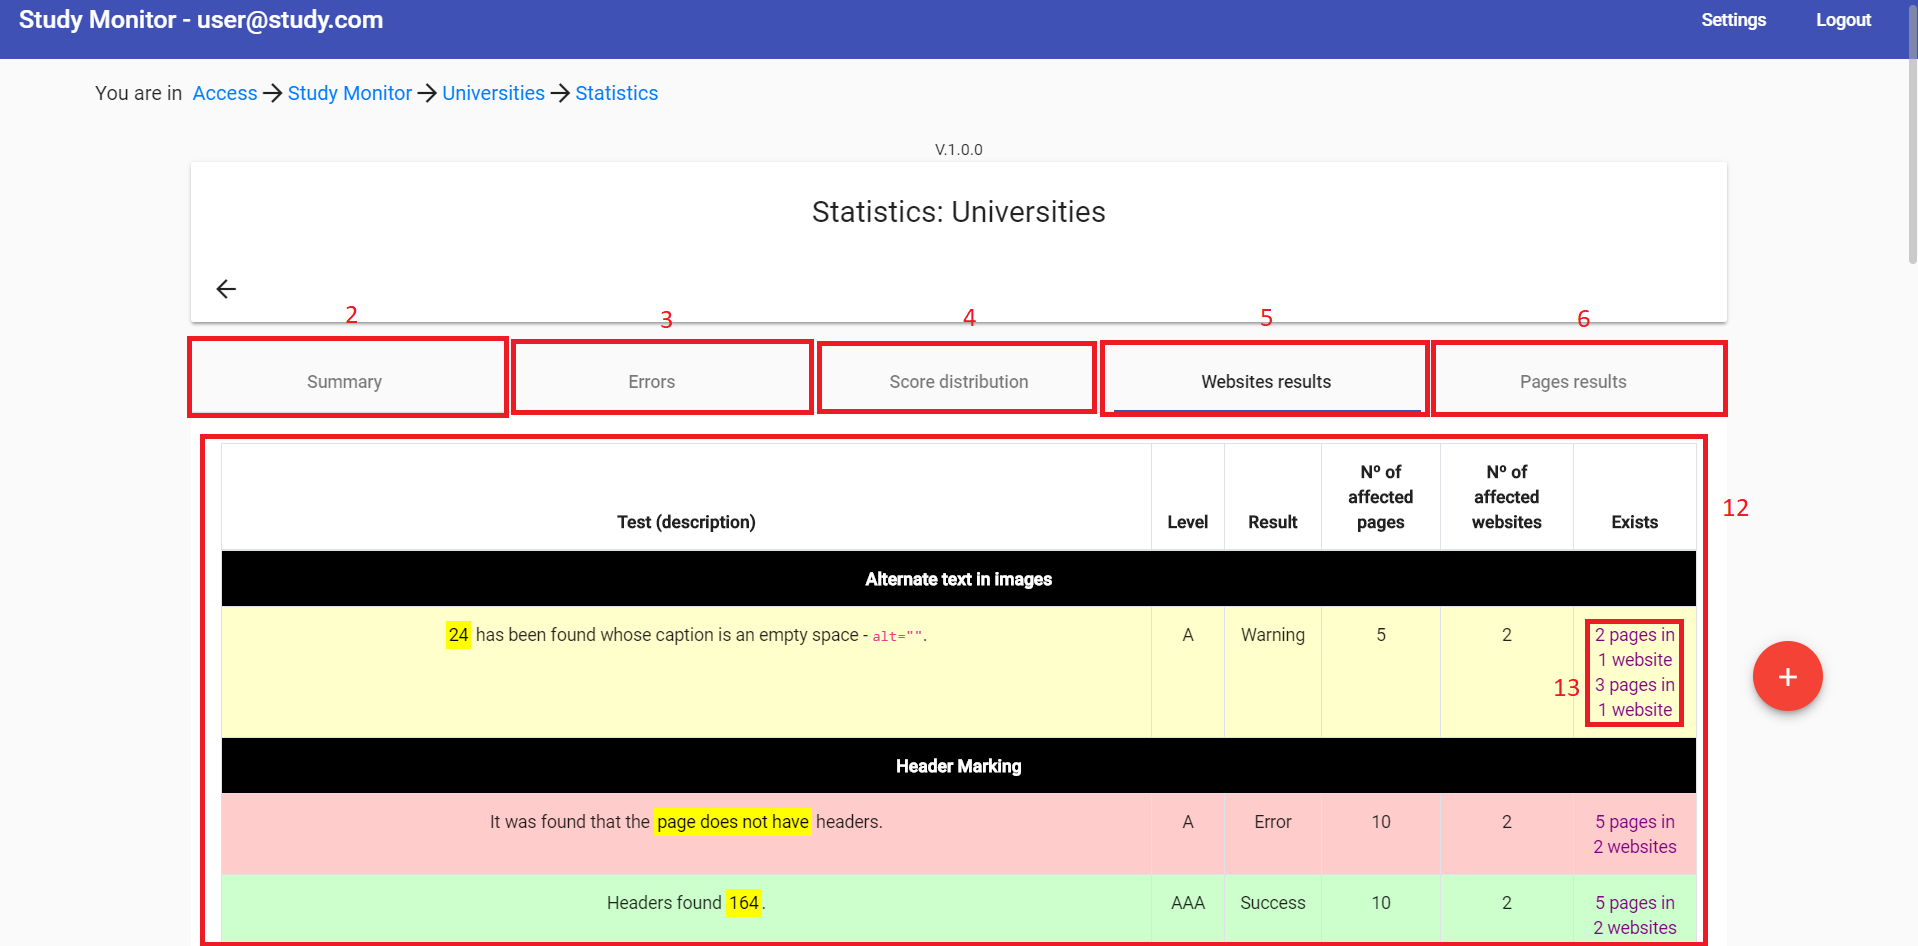
\includegraphics[width=\linewidth]{lib/images/study/study_category_statistics_4.png}
    \caption{Study Monitor category statistics page (cont.)}
    \label{fig:study_category_statistics_page_4}
\end{figure}

\begin{figure}[H]
    \centering
    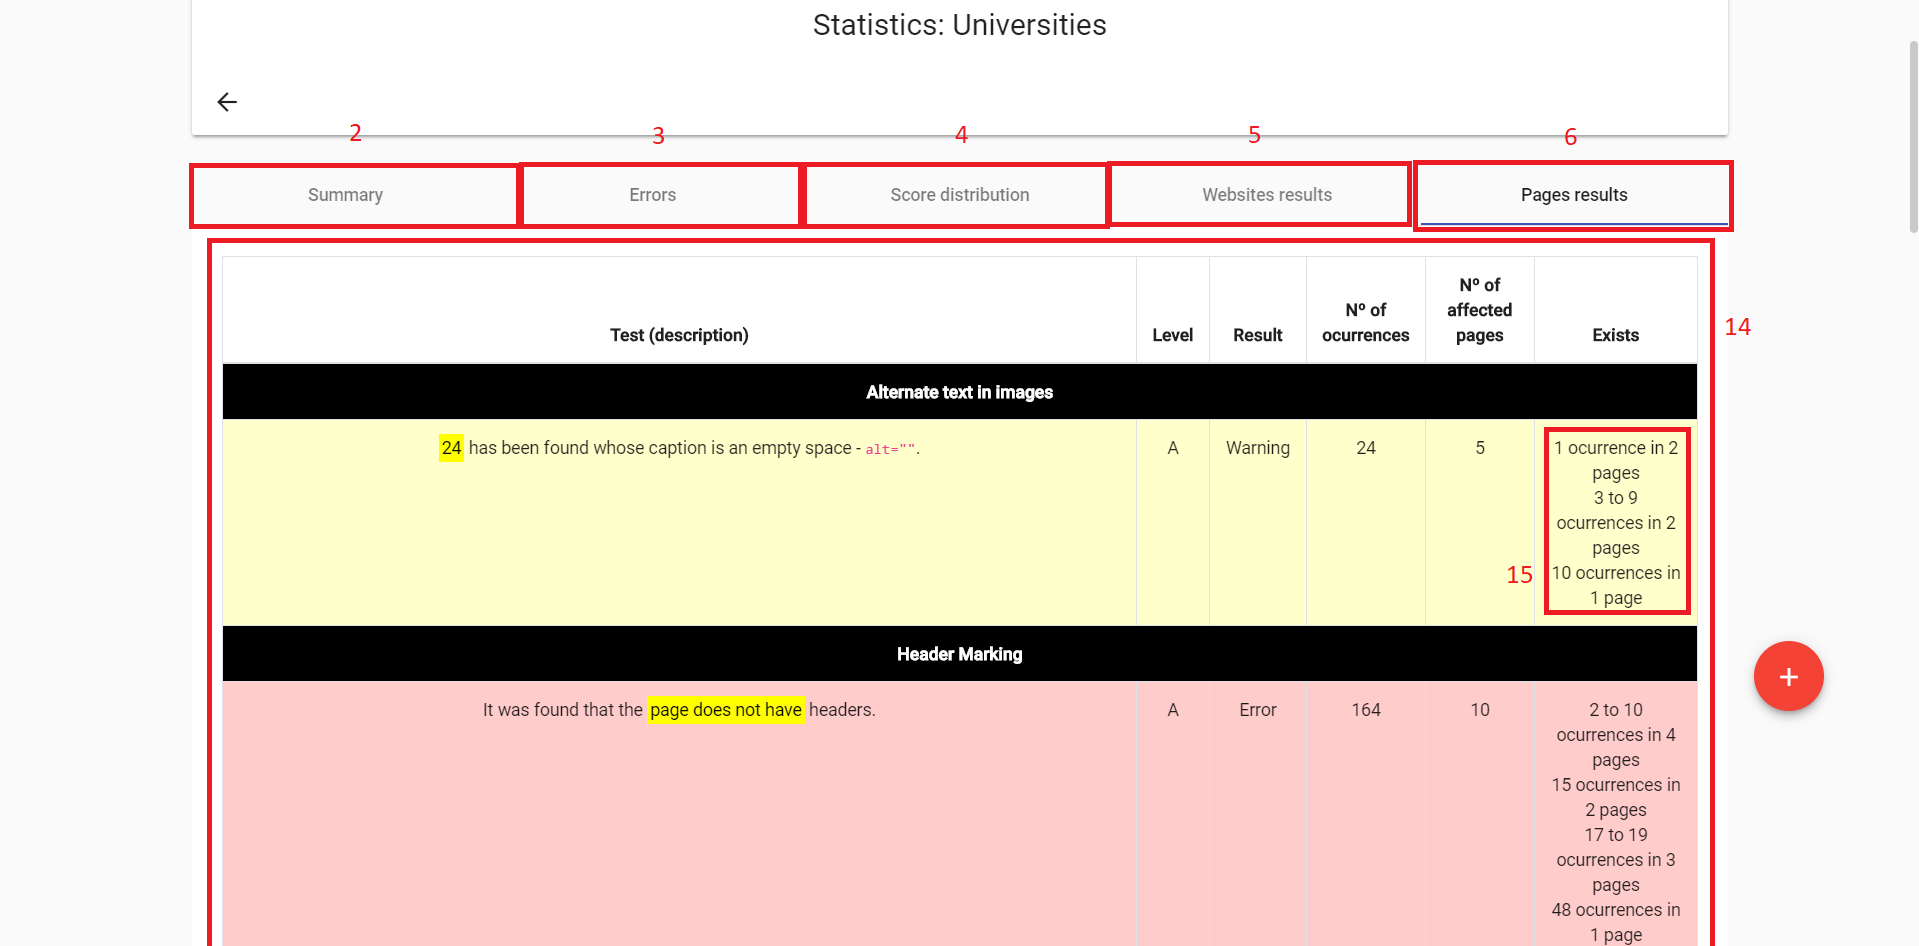
\includegraphics[width=\linewidth]{lib/images/study/study_category_statistics_5.png}
    \caption{Study Monitor category statistics page (cont.)}
    \label{fig:study_category_statistics_page_5}
\end{figure}

\begin{enumerate}
    \item Goes back to the previous page (category page)
    \item Category statistics summary tab
    \item Category errors per conform level tab
    \item Category score distribution tab
    \item Category websites detailed errors tab
    \item Category pages detailed errors tab
    \item Category general statistics
    \item Category pages errors per conform level
    \item Category websites errors per conform level
    \item Category pages score distribution graph
    \item Category websites score distribution graph
    \item Category website detailed errors
    \item Go to ``website errors'' page
    \item Category pages detailed errors
    \item Test occurrences per category page
\end{enumerate}

\section{Website errors page}

Figure \ref{fig:study_website_errors_page}.

\begin{figure}[H]
    \centering
    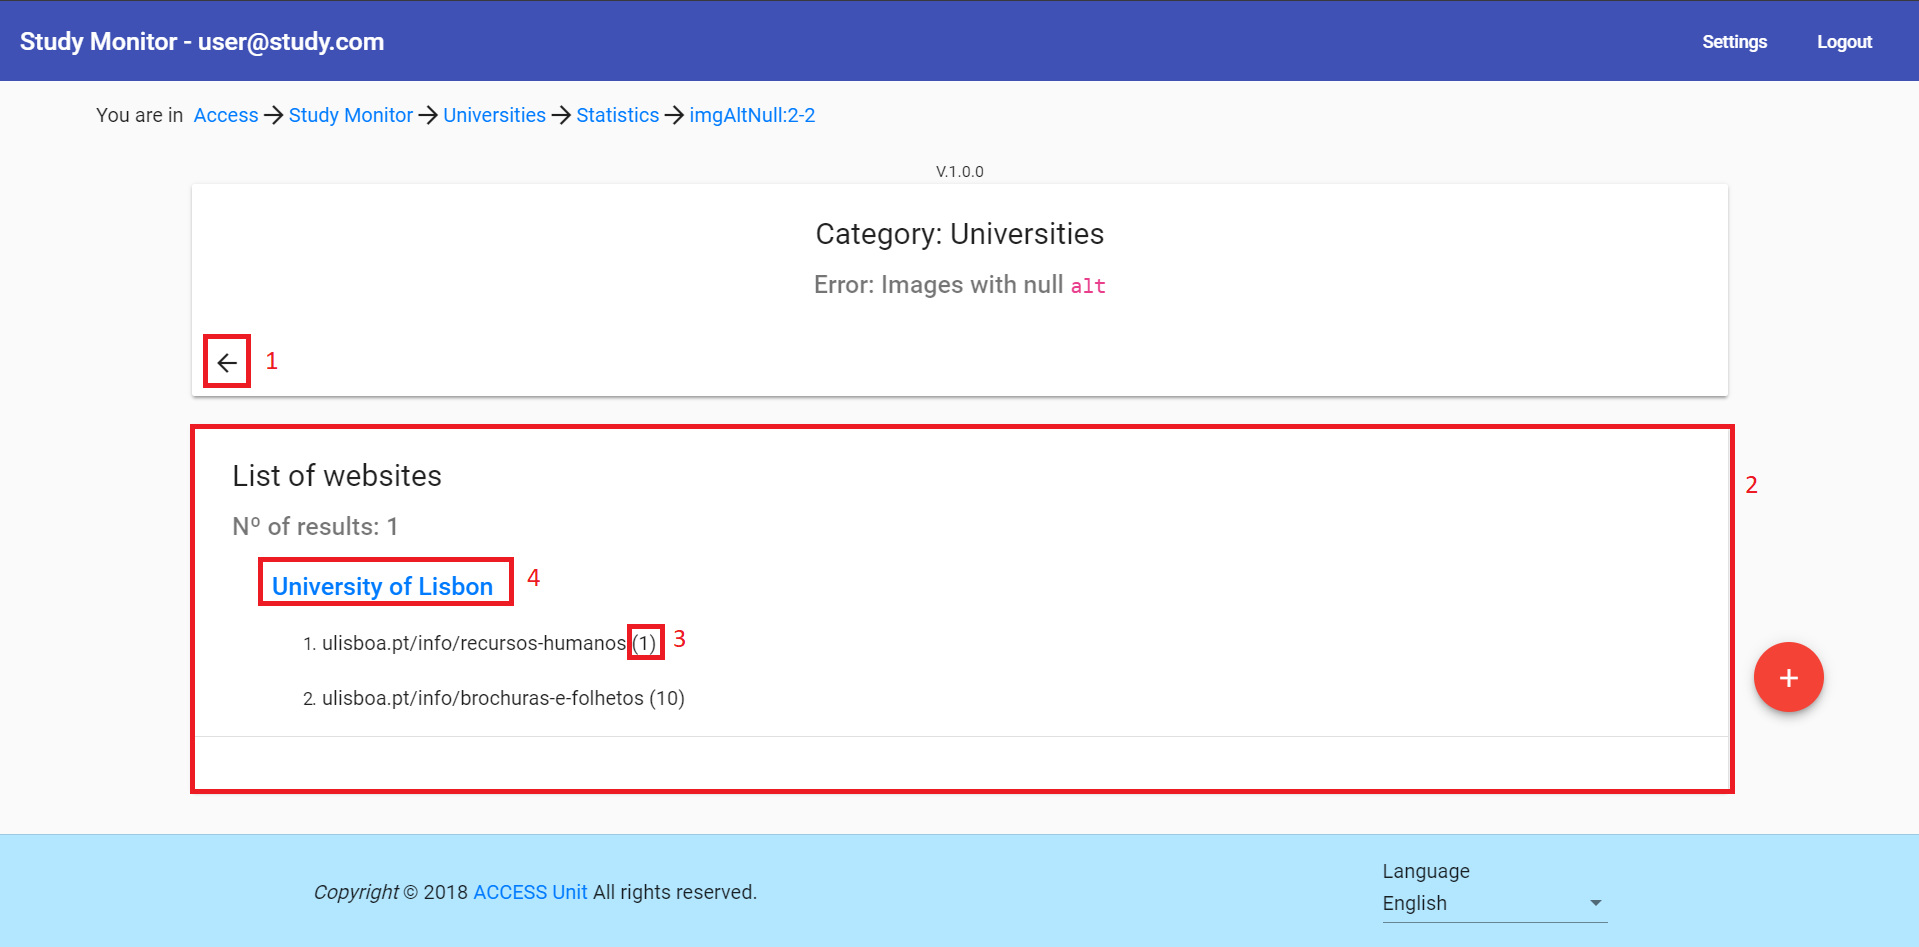
\includegraphics[width=\linewidth]{lib/images/study/study_website_errors_page.png}
    \caption{Study Monitor website errors page}
    \label{fig:study_website_errors_page}
\end{figure}

\begin{enumerate}
    \item Goes back to the previous page (category statistics page)
    \item List of websites with the current test occurrences
    \item Number of occurrences per page
    \item See website information
\end{enumerate}

\section{Website page}

Figures \ref{fig:study_website_page} - \ref{fig:study_website_page_3}.

\begin{figure}[H]
    \centering
    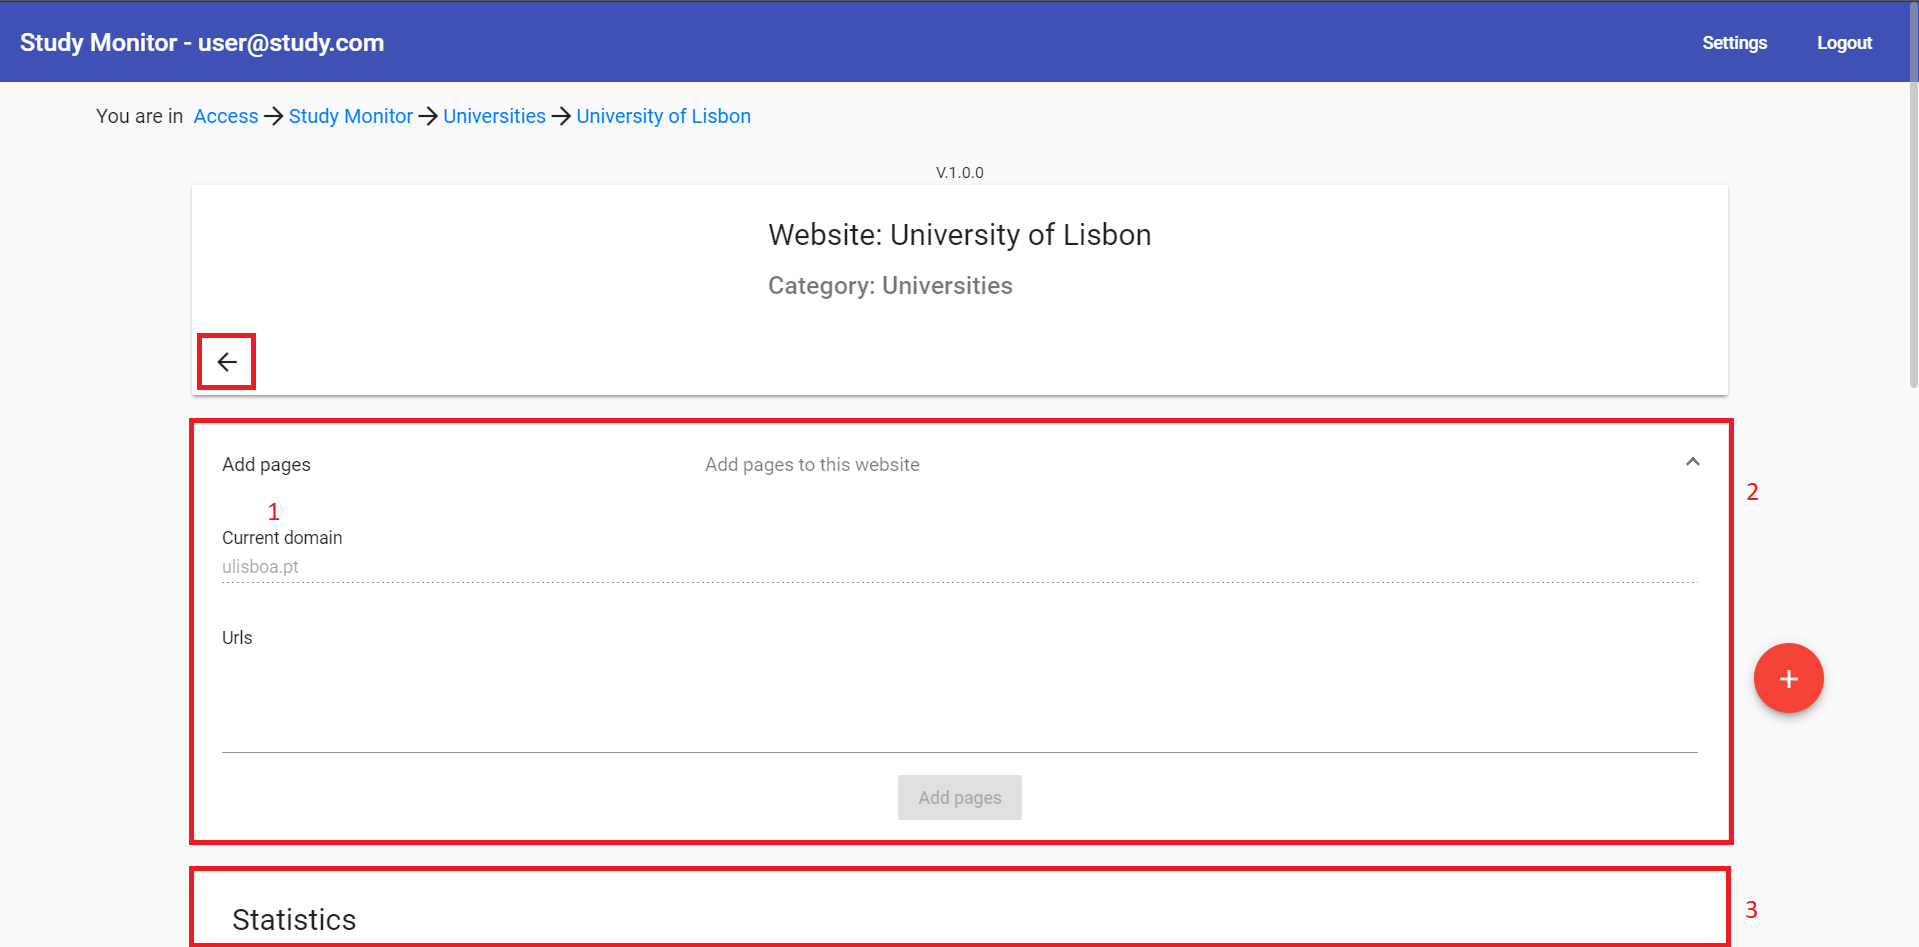
\includegraphics[width=\linewidth]{lib/images/study/study_website_page.png}
    \caption{Study Monitor website page}
    \label{fig:study_website_page}
\end{figure}

\clearpage

\begin{figure}[H]
    \centering
    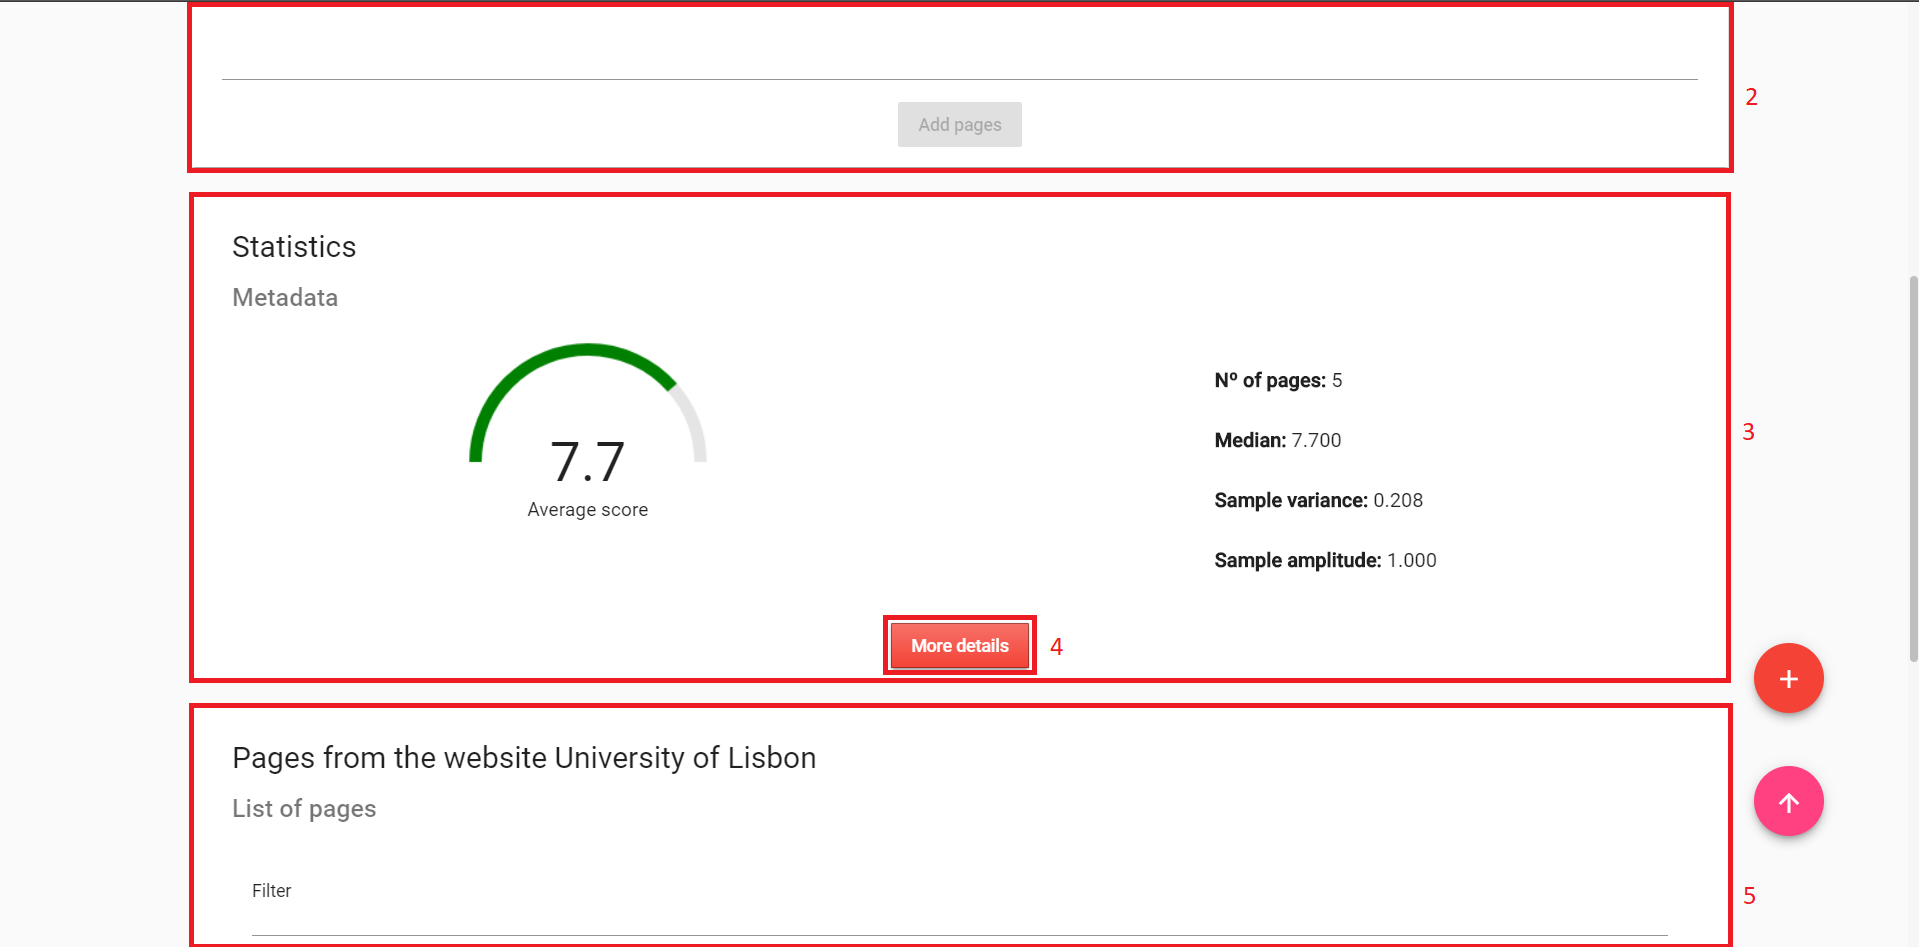
\includegraphics[width=\linewidth]{lib/images/study/study_website_page_2.png}
    \caption{Study Monitor website page (cont.)}
    \label{fig:study_website_page_2}
\end{figure}

\begin{figure}[H]
    \centering
    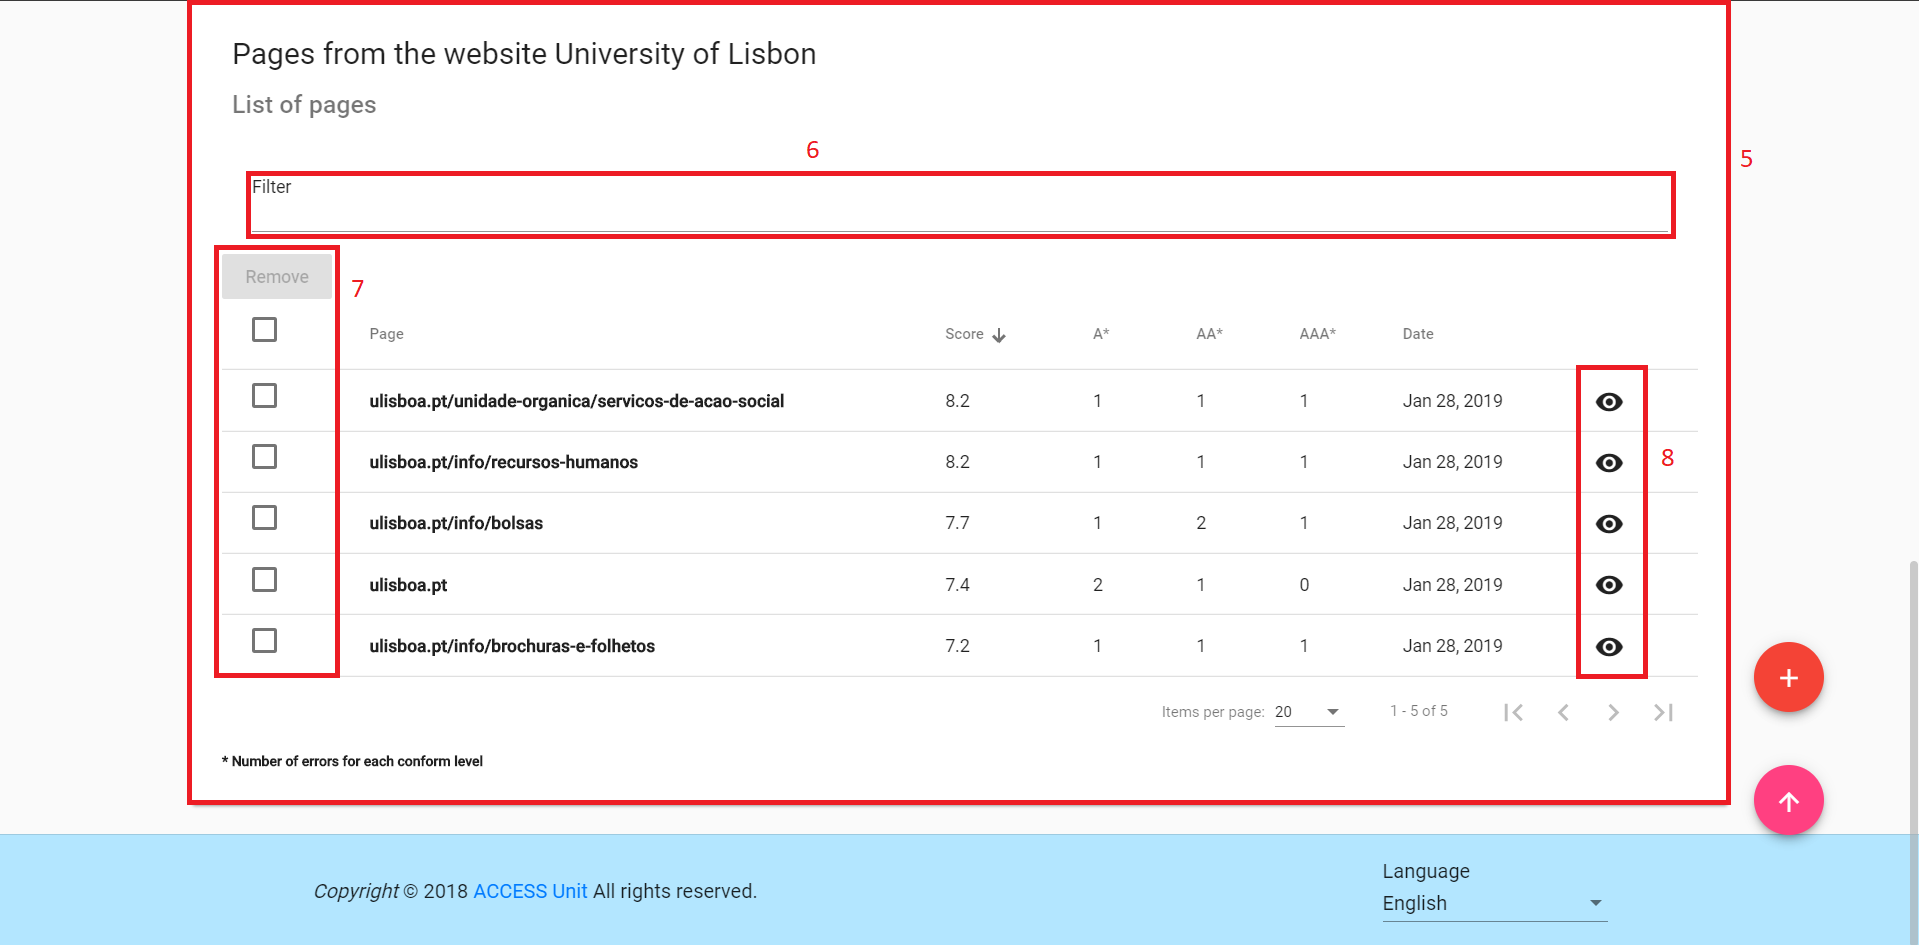
\includegraphics[width=\linewidth]{lib/images/study/study_website_page_3.png}
    \caption{Study Monitor website page (cont.)}
    \label{fig:study_website_page_3}
\end{figure}

\begin{enumerate}
    \item Goes back to the previous page (category page)
    \item Add new pages to the current website form
    \item Website general statistics
    \item Go to ``Category detailed statistics'' page
    \item List of category websites
    \item Website pages filter
    \item Remove pages from the website
    \item See page evaluation results
\end{enumerate}

\section{Website statistics page}

Figures \ref{fig:study_website_statistics_page} - \ref{fig:study_website_statistics_page_3}.

\begin{figure}[H]
    \centering
    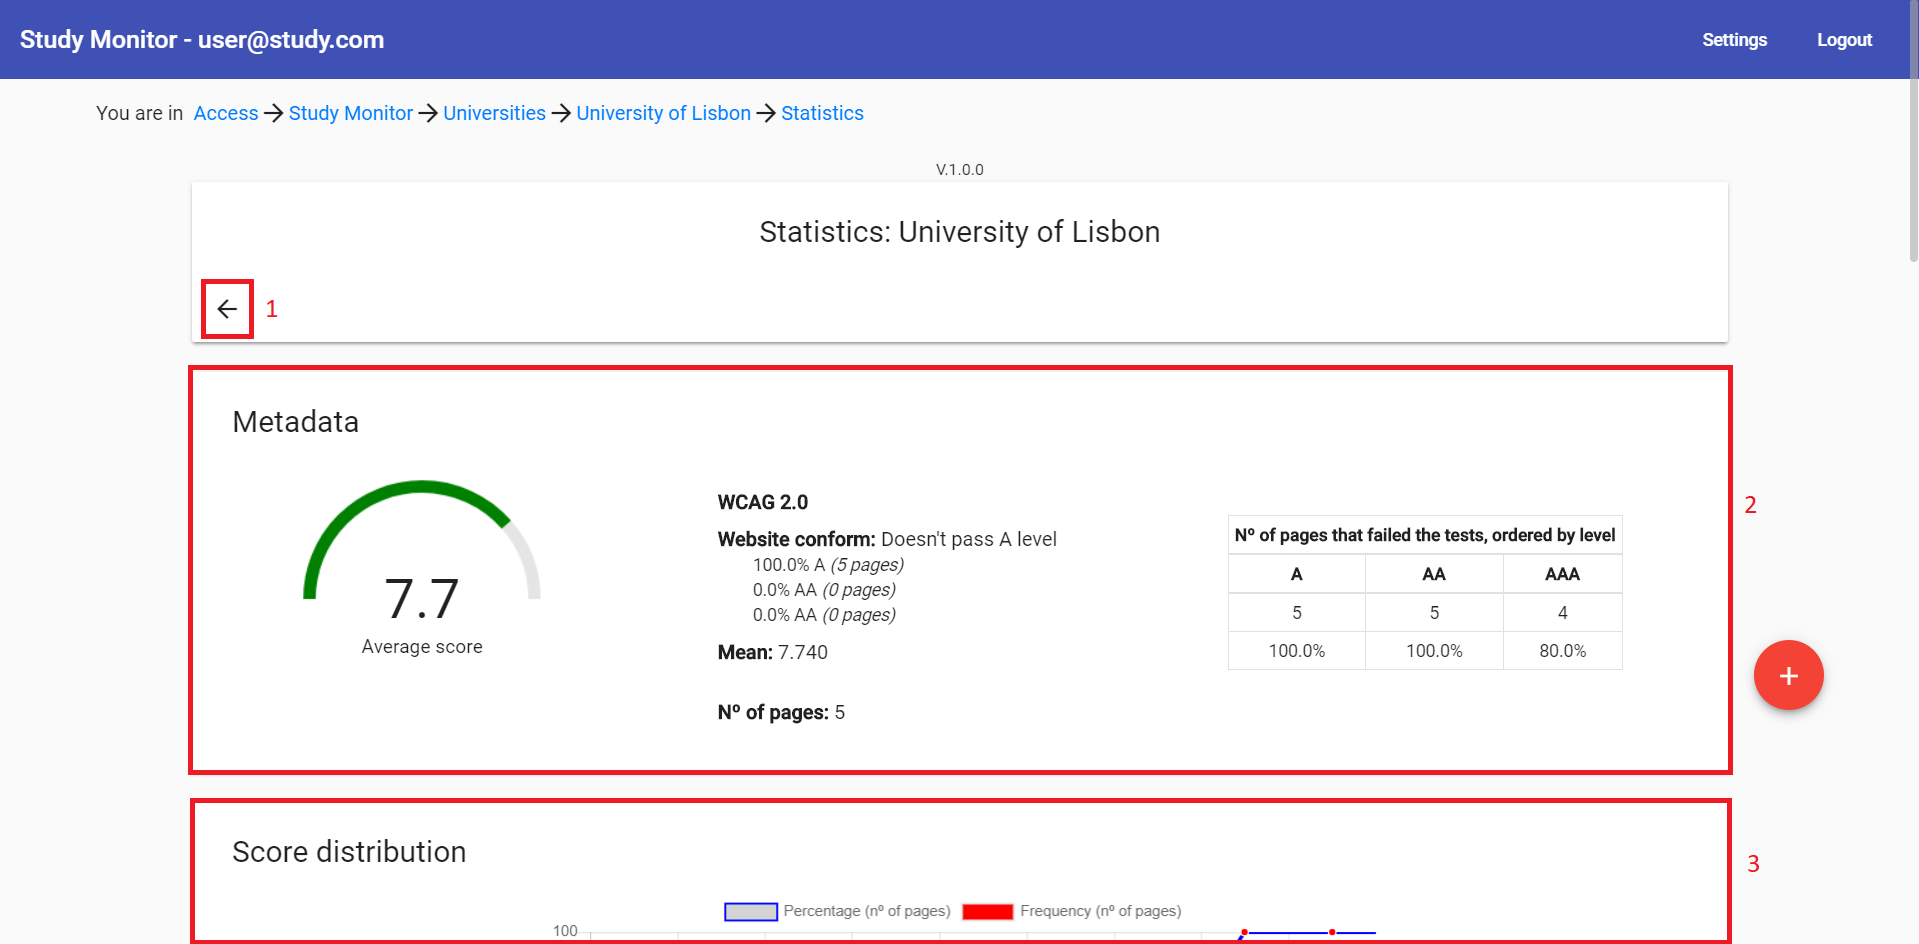
\includegraphics[width=\linewidth]{lib/images/study/study_website_statistics_page.png}
    \caption{Study Monitor website statistics page}
    \label{fig:study_website_statistics_page}
\end{figure}

\clearpage

\begin{figure}[H]
    \centering
    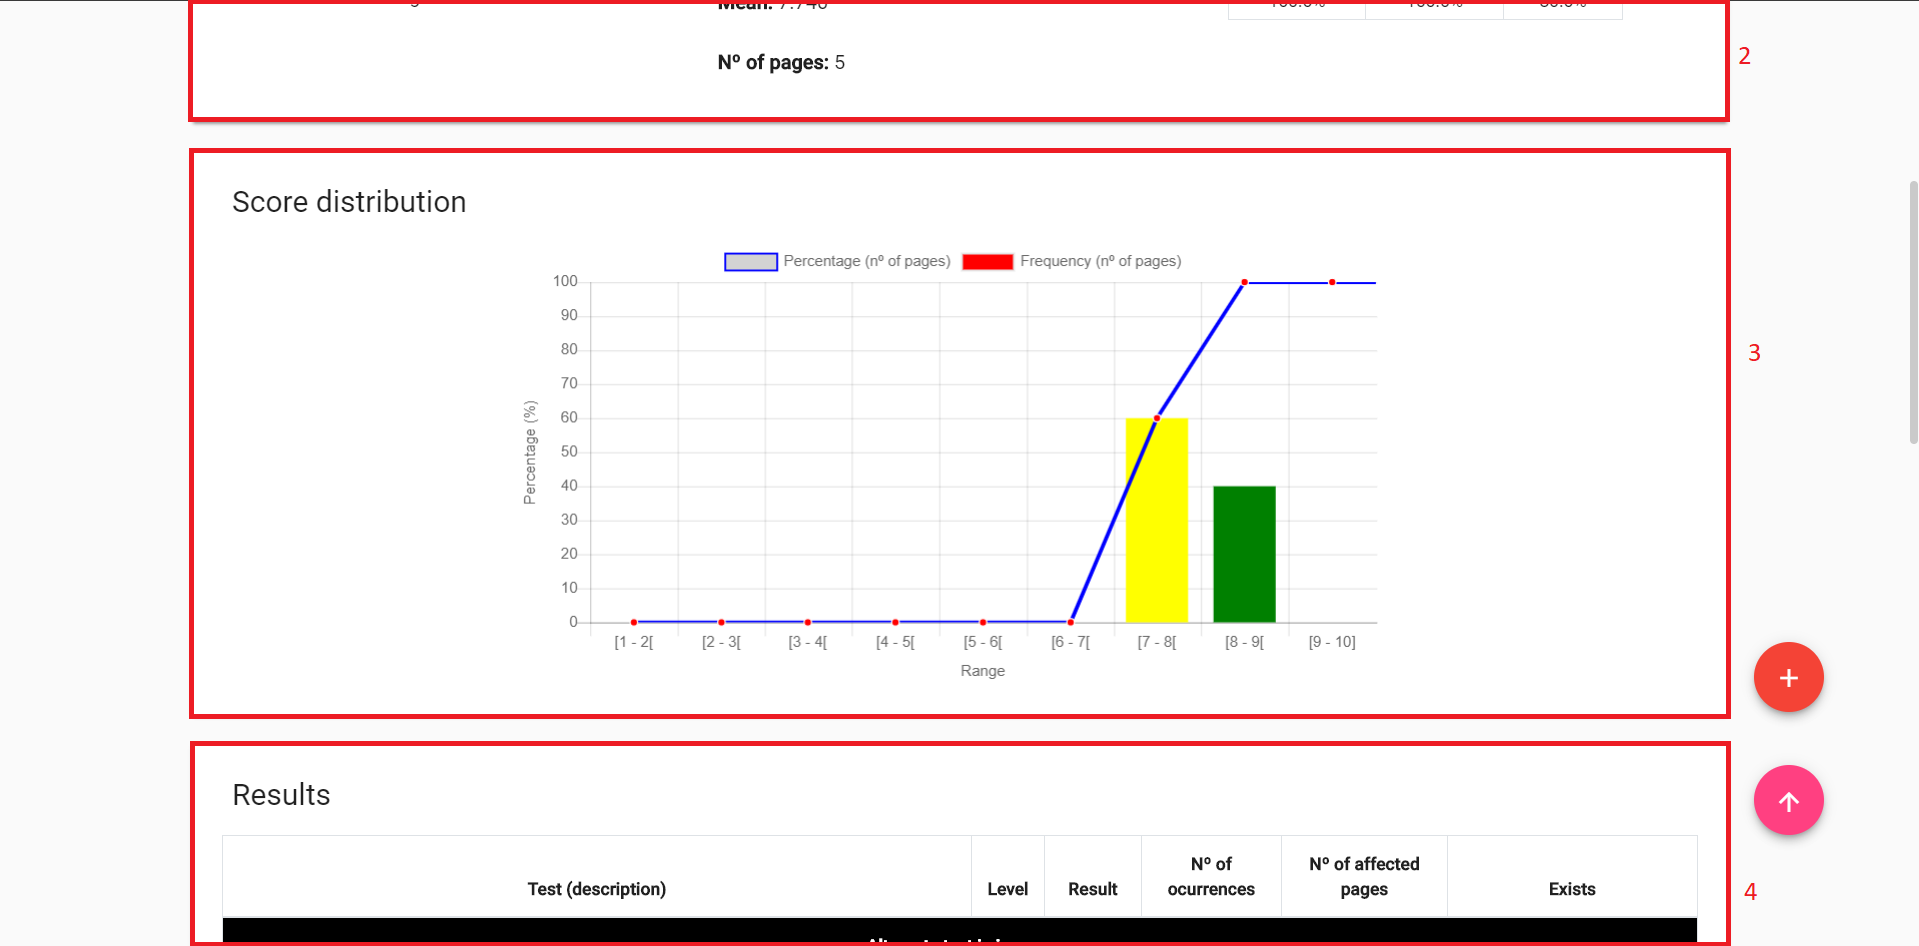
\includegraphics[width=\linewidth]{lib/images/study/study_website_statistics_page_2.png}
    \caption{Study Monitor website statistics page (cont.)}
    \label{fig:study_website_statistics_page_2}
\end{figure}

\begin{figure}[H]
    \centering
    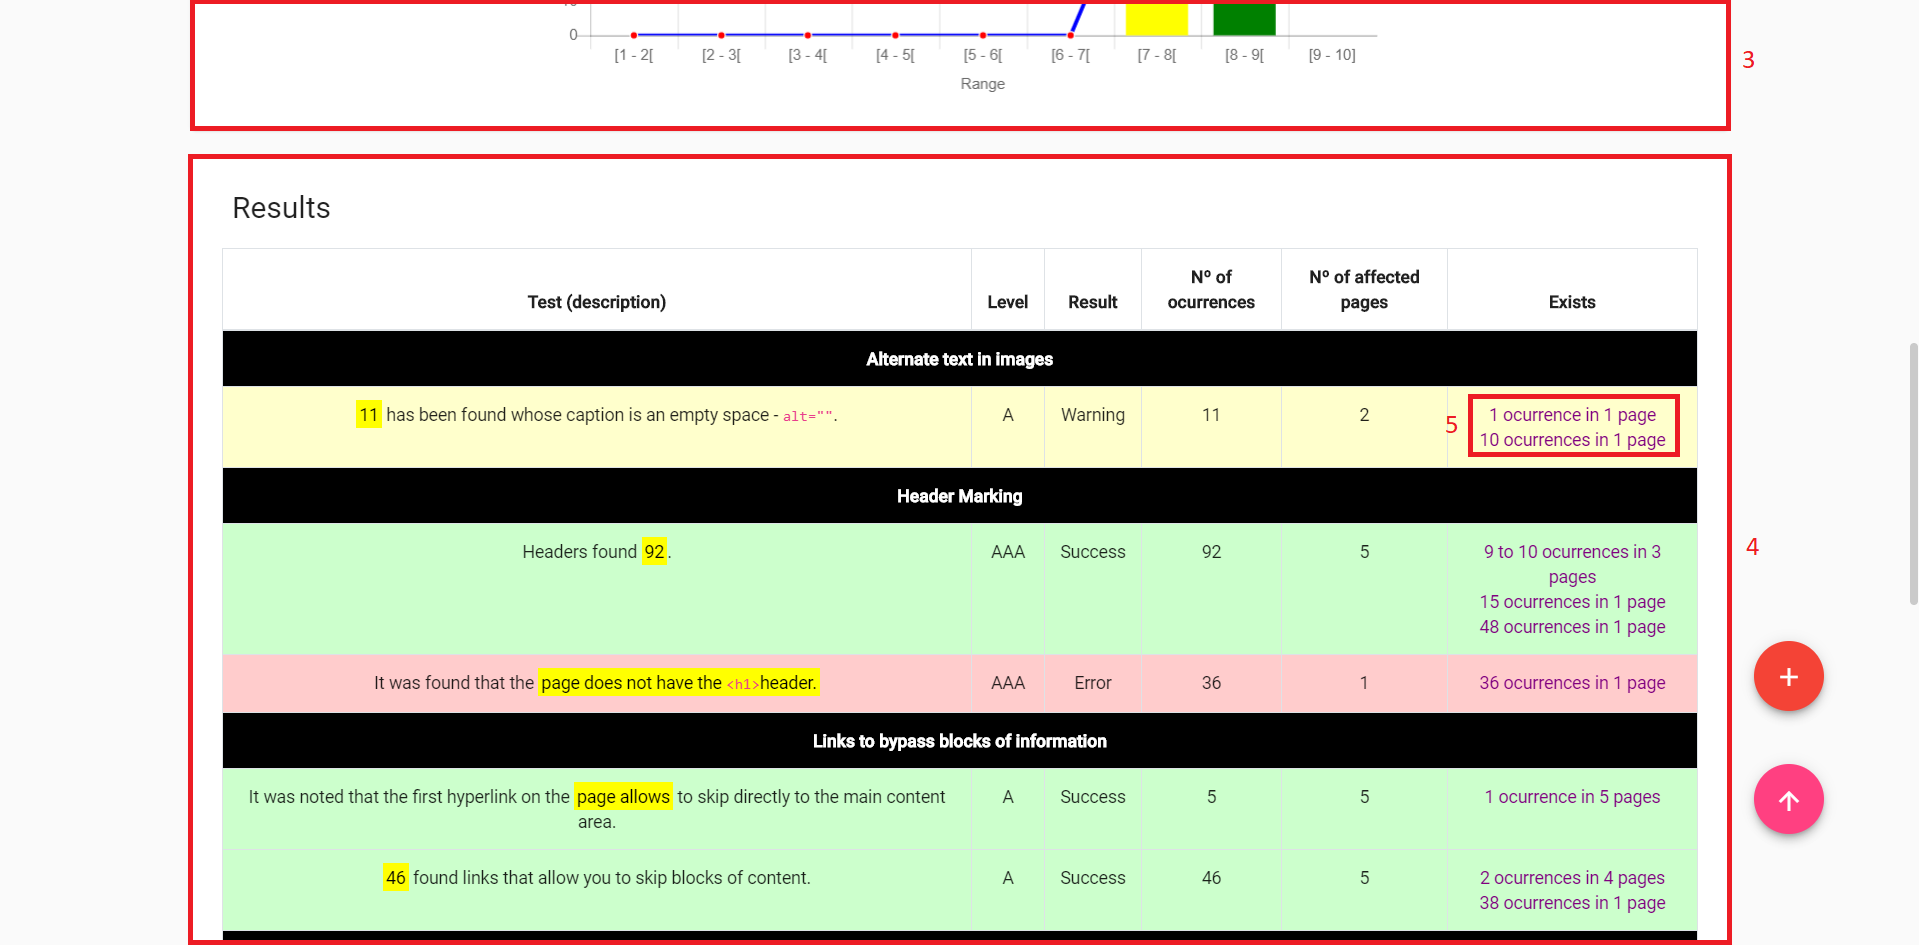
\includegraphics[width=\linewidth]{lib/images/study/study_website_statistics_page_3.png}
    \caption{Study Monitor website statistics page (cont.)}
    \label{fig:study_website_statistics_page_3}
\end{figure}

\begin{enumerate}
    \item Goes back to the previous page (website page)
    \item Website statistics
    \item Website score distribution graph
    \item Website detailed tests table
    \item Go to ``Pages errors'' page
\end{enumerate}

\section{Pages errors page}

Figure \ref{fig:study_pages_errors_page}.

\begin{figure}[H]
    \centering
    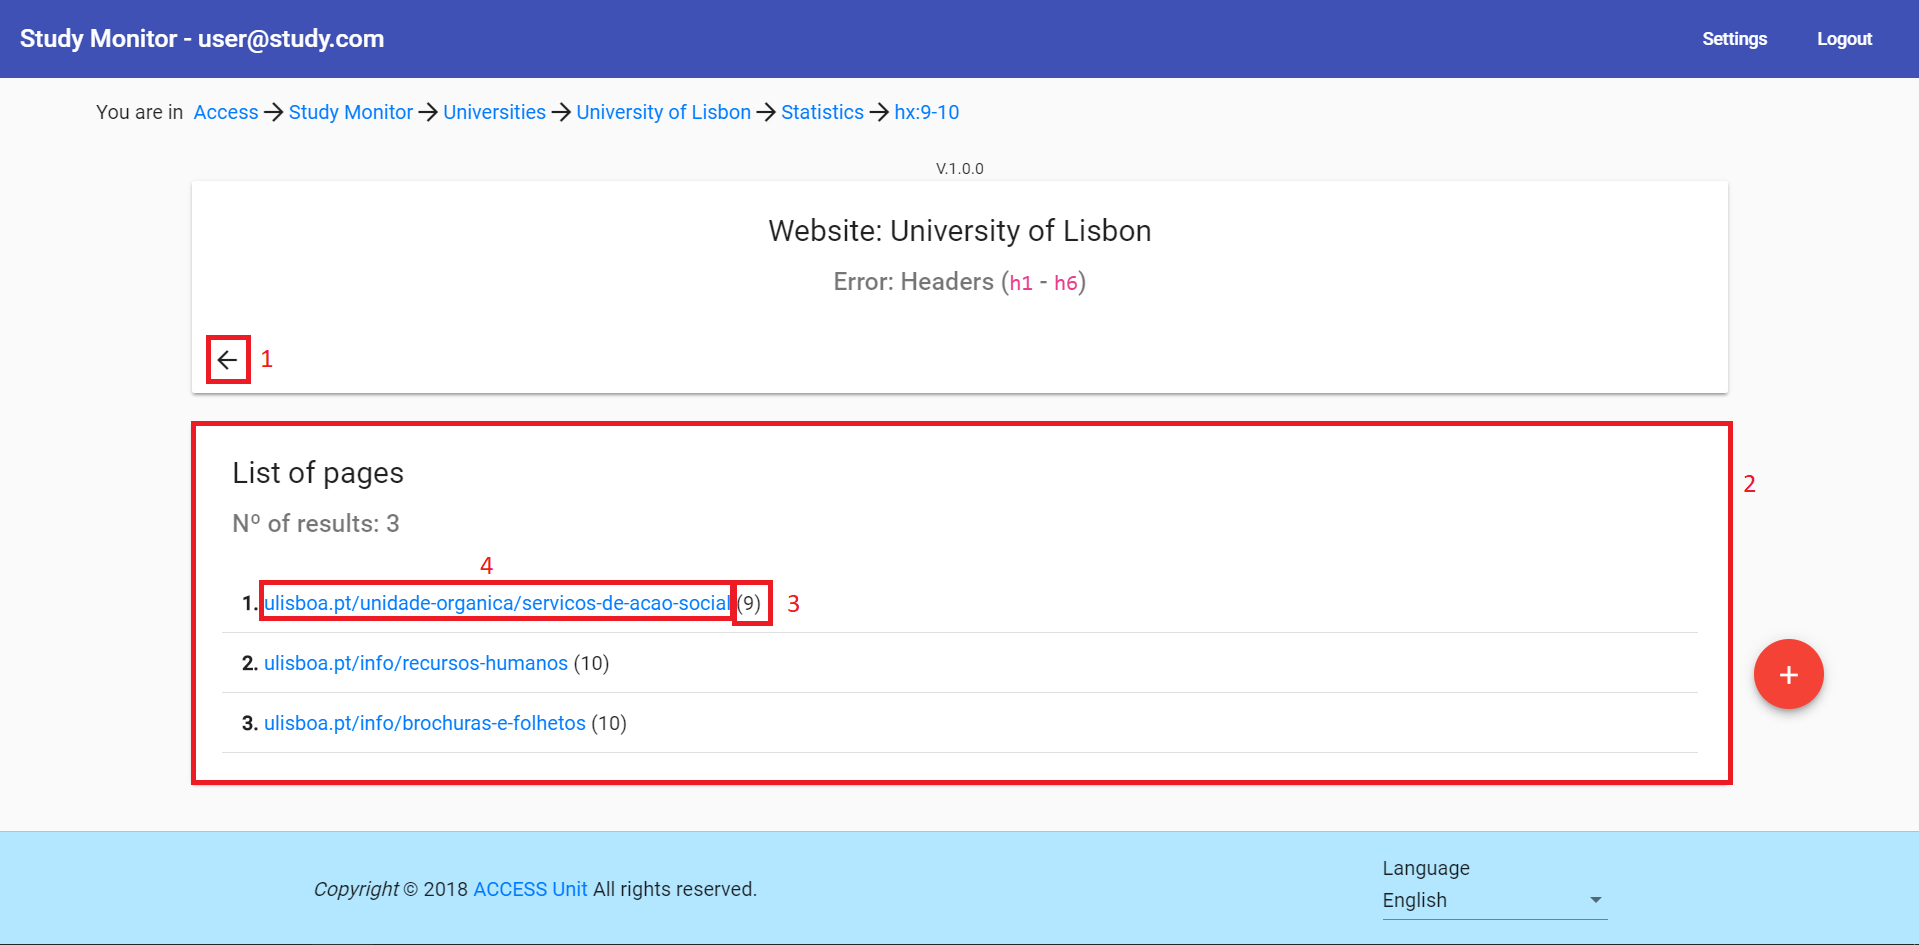
\includegraphics[width=\linewidth]{lib/images/study/study_pages_errors_page.png}
    \caption{Study Monitor pages errors page}
    \label{fig:study_pages_errors_page}
\end{figure}

\begin{enumerate}
    \item Goes back to the previous page (website statistics page)
    \item List of pages with the current test occurrences
    \item Number of occurrences per page
    \item See page evaluation results
\end{enumerate}

\section{Results page}

Check Access Monitor Plus results page, section \ref{sec:amp_results_page}.

\section{Webpage code page}

Check Access Monitor Plus webpage code page, section \ref{sec:amp_webpage_code_page}.

\section{Element result page}

Check Access Monitor Plus element result page, section \ref{sec:amp_element_result_page}.